% Compile with: latexmk -pdfxe -outdir=build
\documentclass[12pt,oneside]{LuThesis}

\title{Saules paneļu efektivitāte Latvijas klimatā}
\author{Viktorija Leimane}

%%% LuThesis deklerācijas
\def\studaplnum{vl16047}
\def\darbvad{Dr. Phys. Andris Jakovičs}
\def\dokfak{\textbf{Fizikas, matemātikas un optometrijas fakultāte}}
\def\recenzents{Dr. Phys.Aivars Vembris}
\def\doktitle{\textbf{Saules paneļu efektivitāte Latvijas klimatā}}
\def\dokfak{\textbf{Fizikas, matemātikas un optometrijas fakultāte}}
\def\dokdate{} % Darba vadītāja parakstīšanas datums
\def\dokdateiesn{} % Darba iesniegšanas datums

%%% Valodas un fonti
\setdefaultlanguage{latvian}
\setotherlanguage{english}
\setmainfont[BoldFont=FreeSerifBold.ttf,ItalicFont=FreeSerifItalic.ttf,BoldItalicFont=FreeSerifBoldItalic.ttf]{FreeSerif.ttf}

\usepackage{graphicx}

%%% Misc
% \usepackage{hyperref}
\usepackage[hidelinks]{hyperref}
\addbibresource{bachelor.bib} % biblatex bibliotēkas fails: bachelor.bib
\usepackage[section]{placeins}

%%% Dokumenta struktūra
\begin{document}

\maketitle

% * Anotācija
\chapter*{Anotācija}
\setcounter{page}{1}
\begin{abstract}
Darba mērķis ir noteikt efektīvāko saules paneļu izvietojuma veidu Latvijas klimatiskajos apstākļos. 
Balstoties uz divu veidu saules paneļiem, kas novietoti piecās dažādās telpiskajās orientācijās Latvijas Universitātes Botāniskā dārza teritorijā, tiek noteikta solāro paneļu efektivitātes atkarība no mainīgiem parametriem:
\begin{enumerate}
\item solāro paneļu tips
\item telpiskā orientācija
\item gada mēnesis
\item meteoroloģiskie apstākļi.
\end{enumerate}

Iegūtie monitoringa rezultāti tiek analizēti kontekstā ar saules izstarojuma intensitāti, paneļu parciālās(?) efektivitātes fizikālo novērtējumu un citu mērījumu rezultātiem.\\

\keywords{Saules enerģijas paneļi, atjaunojamo energoresursu enerģija}
\end{abstract}

\chapter*{Abstract}
\begin{english}
\begin{abstract}
The aim of this thesis is to determine optimal solar panel arrangement for the climatic conditions of Latvia.
By studying two types of solar panels placed in five different spatial orientations in the University of Latvia Botanical Garden area, the dependency of solar panel efficiency on following variable parameters is established:
\begin{enumerate}
\item Type of solar panels (JA or LG)
\item Spatial orientation (W.13, E.13, S.13, S.40, S.90)
\item Month of year (january - april)
\item Meteorological conditions (solar irradiance and clouds)
\end{enumerate}

The results of the monitoring are analysed in the context of solar irradiance intensity, the physical assessment of the potential efficiency of the panels and the results of other measurements.
The results show that the optimal parameters are LG panel at a direction south 40 degree angle. The study data analysis tool is available in \url{https://github.com/chararchter/solR}.

\keywords{Solar panels, renewable energy}
\end{abstract}
\end{english}

%* Saturs
\tableofcontents

%* Apzīmējumu saraksts
\chapter*{Apzīmējumu saraksts}
\addcontentsline{toc}{chapter}{Apzīmējumu saraksts}
\noindent 
\textbf{Klimats}\\
TSI - Kopējais saules apstarojums, $\textrm{Wm}^{-2}$\\
SSI - Saules spektrālais apstarojums, $\textrm{Wm}^{-2}\textrm{nm}^{-1}$\\
% $G_{sc}$ - Solārā konstante, $\textrm{Wm}^{-2}$\\
%Photovoltaic power potential
TIM - Kopējā apstarojuma novērotājs\\
GHI – Globālais horizontālais apstarojums,  $\textrm{kWh/m}^2$\\ %Global horizontal irradiation
DHI – Difūzais horizontālais apstarojums,  $\textrm{kWh/m}^2$\\ 
DNI – Tiešais normālais apstarojums, $\textrm{kWh/m}^2$\\ %Direct normal irradiation
CMF - Mākoņu modifikācijas reizinātājs\\
AU - astronomiskā vienība\\  %astronomical unit
\textbf{Saules kustības leņķi}\\
$\theta$ - staru krišanas leņķis uz saules paneli\\
$\delta$ - Saules deklinācija -- leņķis starp virzieniem uz Sauli un debess ekvatoru solārajā pusdienlaikā.\\
 $\phi$  - ģeogrāfiskais platums; pozitīvs Z virzienā.\\
$\beta$  - paneļa slīpums -- leņķis starp Saules paneļa virsmu un horizontāli.\\
$\gamma$ - paneļa azimuts -- leņķis starp virsmas normāles projekciju uz horizontālo  plakni un D virzienu.\\
$\omega$ - solārais stundu leņķis -- leņķis starp Saules stara virziena projekciju uz horizontālo plakni un D virzienu; negatīvs no rīta.\\
\textbf{Saules paneļi}\\
PV - fotoelektriskais elements\\ %fotogalvanisks?
Si - silīcijs\\
P - jauda, 	W\\
Pmax - maksimālā jauda, W\\
PVOUT – Saules fotoelementa potenciālā jauda, $\textrm{kWh/kWp}$\\ 
%Photovoltaic power potential
E$_{norm}$, $\textrm{kWh/m}^2$ - enerģija normēta uz saules paneļa laukuma vienību.\\
\textbf{Debespuses}\\
A - austrumi\\
R - rietumi\\
D - dienvidi\\

%* Ievads
\chapter*{Ievads}
\addcontentsline{toc}{chapter}{Ievads}
Apvienoto Nāciju Organizācijas Klimata konferencē Parīzē 2015. gada decembrī daudzas pasaules valstis vienojās ierobežot globālo sasilšanu zem 2 ºC salīdzinājumā ar pirmsindustriālo laikmetu.
%, tāpēc ES ir apņēmusies līdz 2030. gadam samazināt siltumnīcefekta gāzu emisijas vismaz par 40\% salīdzinājumā ar 1990. gada līmeni.
Tāpēc Eiropas Savienībā noteikts dalībvalstīm saistošs mērķrādītājs  –  vismaz 32\%  atjaunojamās enerģijas īpatsvars līdz 2030. gadam \cite{ES}.

Ne mazāk būtiska ir atjaunojamo energoresursu loma energoapgādes neatkarības un drošības veicināšanā, tehnoloģiju attīstībā un inovācijās, vienlaikus sniedzot labumu videi un sabiedrībai, kā arī nodrošinot svarīgus priekšnosacījums nodarbinātībai, reģionālajai attīstībai un elektrības nodrošināšanai grūti pieejamās vietās \cite{ES}.

Dažādu pieejamo atjaunojamo resursu - Saule, vējš, zeme, ūdens - starpā Saules enerģija ir viens no kandidātiem klimata pārmaiņu un to seku mazināšanai un efektīvas energoapgādes nodrošināšanai. Pēdējā desmitgadē veiktās investīcijas Saules enerģijas izmantošanā manifestējās inovācijās saules paneļu ražošanā, un gala rezultātā tie ir kļuvuši efektīvāki un finansiāli pieejamāki patērētājiem, piemēram, rakstā \cite{researchOpp} norādīts, ka silīcija saules paneļu cena sastāda mazāk nekā 30\% no kopējām saules paneļu sistēmas uzstādīšanas izmaksām un to saražotā enerģija atmaksājas vidēji trīs gadu periodā.

Tomēr bez klimata to efektivitāti ietekmē arī daudzi citi faktori, to skaitā telpiskā orientācija.

Šī pētījuma \textbf{mērķis} ir analizēt un praktiski pārbaudīt divu tipu (JA un LG) saules paneļu efektivitāti atšķirīgos telpiskās orientācijās risinājumos -- pētītas trīs dažādu virzienu (dienvidi, rietumi, austrumi) un trīs leņķu (13, 40, 90) paneļu grupas -- un tiek salīdzināta to piemērotība Latvijas klimatiskajiem apstākļiem.

\textbf{Darba uzdevumi}
\begin{itemize}
\item Ievākt, atlasīt un analizēt saules paneļu datus.
\item Izveidot iespējami automatizētu datu apstrādes sistēmu R valodā ilgtermiņa montioringa vajadzībām.
\item Salīdzināt paneļu efektivitāti mēnešu un gada laikā atbilstoši to parametru (paneļu tipa un telpiskās orientācijas) apakšklasēm.
% \item Balstoties uz ilgtermiņa saules izstarojuma monitoringu, novērtēt saules paneļu saražoto enerģiju no fizikālajiem apsvērumiem.
\item Novērtēt datu kvalitāti no fizikālo apsvērumu un citu mērījumu viedokļa.
\end{itemize}

\textbf{Darba struktūra}\\
Darba pirmo daļu veido literatūrā pieejamo Saules apstarojuma novērtējumu raksturojums un apskata par Saules redzamo pārvietošanās pie debess sfēras diennakts laikā janvāra un aprīļa mēnešos. Otrajā daļā aplūkota saules paneļu uzbūve un darbības princips, kā arī apskatīta sistēmas shēma un saues paneļu konkrētās instalācijas LU Botāniskajā dārzā parametru raksturojums.
Trešā daļā ir aprakstīti iegūtie rezultāti, tie ir salīdzināti savā starpā, ar cita saules paneļa uzstādījuma mērījumu rezultātiem un 


ar eksperimentālā poligona meteostacijas datiem par solāro apstarojumu šajā laika periodā.


% un lai to analīzi veiktu ir darīti uzdevumi
% uzstādīti paneļi (profesionāļi to darīja)
% Ievākti un analizēti dati
% Datu kvalitātes novērtējums
% novērtēt vai iegūtie resultāti ir ticami

% citos klimatiskajos apstākļos līdzīgas analīzes ir veiktas ko var iegūt dažādās klimatiskajās zonās 
% pierakstīt par pv paneļu darbību un efektivitāti
% aprakstīt ko tu darīji, lai pēc iespējas automatizētu datu apstrādes sistēmu
% kādus datus uzkrāj kādā attēlojumā
% datu menedžmentu aprakstīt
% % TEORIJAS KOPSAVILKUMS
Vispirms tiek aplūkota Saules emitētā starojuma daba un ģeometriskie apsvērumi - virziens, no kura staru kūlis sasniedz virsmu, leņķis uz virsmas un laika gaitā saņemtais starojuma daudzums. Tiek apskatīta atmosfēras ietekme uz virsmas saņemto saules starojumu, un tās praktiskā nozīme, apstrādājot pieejamos Saules starojuma datus, lai aprakstītu radiācijas gadījumus uz virsmas dažādās orientācijās.

% * Literatūras apskats
\chapter{Literatūras apskats}
% \section{Definīcijas}
\noindent \textbf{Saules plankums} - magnētiskās plūsmas koncentrācija bipolāros klāsteros vai grupās, kas novērojama kā tumšs plankums uz Saules fotosfēras.\\
\textbf{Saules plankumu cikls} - aptuveni 11 gadus ilga kvaziperiodiska variācija saules plankuma skaitlī. Magnētiskā lauka polaritātes modelis mainās ar katru ciklu.\\
\textbf{Saules plankuma skaitlis} - Dienas saules plankuma aktivitātes indekss (R), definēts kā $R = k(10 \cdot g + s)$, kur
s - individuālo plankumu skaits;
g - saules plankumu grupu skaits;
k - observatorijas faktors.\\
\textbf{SSI} - saules spektrālais starojums vai spektra enerģijas blīvums - saules jaudas izkliede uz virsmas laukuma vienību.\\
% total solar irradiance (TSI) - Solar energy per unit time over a unit area perpendicular to the Sun’s rays at the top of Earth’s atmosphere.
\textbf{TSI} - Saules starojuma absolūtās intensitātes mērījums integrēts visā saules enerģijas diskā un visā saules enerģijas spektrā.\\
% Laboratory for Atmospheric and Space Physics, University of Colorado (2019)
% \\http://lasp.colorado.edu/home/sorce/reference/glossary/
\textbf{Izstarojums} - starojuma avota jaudas incidents uz virsmas laukuma vienību.\\ %Irradiance
\textbf{Saules diennakts kustība} (diurnal motion) - Debess spīdekļu redzamā pārvietošanās pie debess sfēras (rotācija ap pasaules asi) diennakts laikā.\\ %Diurnal motion
% Tās faktiskais cēļonis ir Zemes rotācija ap asi. Diennakts kurstībā visi debess spīdekļi pārvietojas pa debess paralēlēm.
Beam Radiation - the solar radiation received from the sun without having been scattered by the atmosphere (also known as direct solar radiation)
Diffuse Radiation - the solar radiation received from the sun after its direction has been changed by scattering by the atmosphere
\input{tex/literatura}
\section{Saules apstarojums}

Lielākā daļa Saules emitētās enerģijas tiek saražota kodolreakcijās fotosfērā. 
Kopējais saules apstarojums (TSI) raksturo Saules starojuma absolūto intensitāti,
enerģiju uz virsmas perpendikulāri starojuma izplatīšanas virzienam 1 AU attālumā no Saules, integrēta visā saules enerģijas diskā un visā saules enerģijas spektrā. \cite{ThermalProcesses} TSI vērtībai novērojama aptuveni 11 gadus ilga periodiska variācija, kas korelē ar saules plankumu skaitli (\ref{fig:TSI_misijas}. att.)  un norāda uz solārās radiācijas izmaiņām, kas ietekmē saņemto solārās enerģijas apjomu uz Zemes atmosfēras augšējiem slāņiem. Papildus ir noderīgi zināt saņemtā starojuma spektrālo sadalījumu (SSI) -- ~\ref{fig:SSI}. attēlā redzams, ka aptuveni puse starojuma tiek saņemta 380 -- 780 nm diapazonā, kas padara iespējumu no tā iegūt enerģiju ar saules paneļu paņēmienu.

TSI novērojumi no kosmosa tiek veikti kopš 1978. gada un instrumentu specifikas dēļ iegūtas dažādas absolūtās vērtības (\ref{fig:TSI_misijas}. att.), tāpēc šī fizikālā lieluma tikai daļēji pārkājušos novērojumu laikrindu apvienošana kompozītā ir gan zinātnisks, gan statistisks izaicinājums un neviens kompozīts (piemēram, PMOD, ACRIM, IRBM) līdz šim nav guvis konsensu solārā apstarojuma pētnieku kopienā.

\begin{figure}[h]
    \centering
    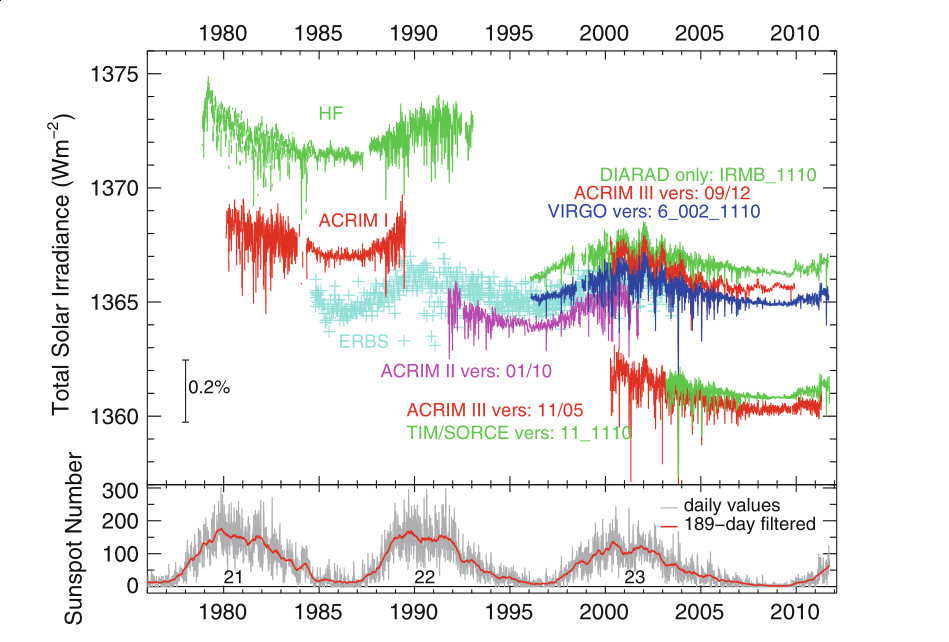
\includegraphics[width=0.6\linewidth]{figures/misc/TSI_misijas.png}
    \caption{Salīdzinājums dienā vidējotiem saules kopējā apstarojuma datiem no dažādām misijām un Saules plankuma skaitlis, lai ilustrētu solārās aktivitātes variabilitāti trīs ciklos. \cite{Frohlich2012}}
    \label{fig:TSI_misijas}
\end{figure}

% \begin{table}[h]
%     \caption{TSI mērījumu vēsture} % uzrakstīt kādu absolūto TSI izmērīja vai norādīt uz grafiku?
%     \begin{center}
%     \begin{tabular}{| r | c | l |}
%     \hline
%     radiometrs & misija & darbības laiks \\ \hline
%     Hickey-Frieden & NIMBUS-7 & 1978--1992  \\ \hline
% 	ACRIM I & Solārā Maksimuma Misija (SMM) & 1980--1989 \\ \hline
% 	ACRIM  & Zemes Radiācijas Budžeta Satelīts (ERBS) & 1984--2003 \\ \hline
% 	ACRIM II & Augšējās Atmosfēras Izpētes Satelīts (UARS) & 1991--2001 \\ \hline
% 	VIRGO & Solārā un Heliosfēras observatorija (SOHO)& 1996--pašlaik \\ \hline
% 	ACRIM III & ACRIMSAT  & 2000--pašlaik \\ \hline
% 	TIM & Saules Radiācijas un Klimata Eksperiments (SORCE) & 2003--pašlaik\\ \hline
%     \end{tabular}
%     \end{center}
%     \label{tab:radiometers}
% \end{table}

Par labāko saules apstarojuma mērījumu reprezentāciju tiek uzskatīti TIM instrumenta dati mēraparāta uzbūves (atšķirībā no citiem radiometriem TIM precizitātes apertūra atrodas tuvu dobumam un redzeslauku bloķējošā apertūra ir pie instrumenta ieejas) un augstās precizitātes -- nenoteiktība tiek novērtēta esam mazāk nekā $0.014\textrm{Wm}^{-2}\textrm{yr}^{-1}$ un precizitāte ar $0.48\textrm{Wm}^{-2}$ \cite{TSIdata} -- dēļ, tāpēc šajā darbā grafiki balstās uz šiem mērījumiem, pēc kuriem absolūtā kopējā saules apstarojuma vērtība ir $1360.8 \pm 0.5 \textrm{Wm}^{-2}$.\cite{Frohlich2012}

\begin{figure}[h]
    \centering
    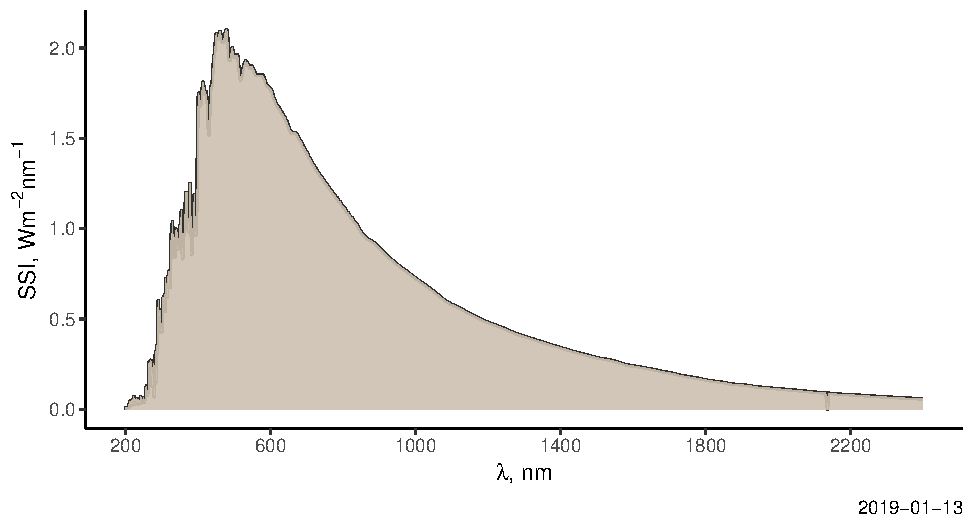
\includegraphics[width=\linewidth]{figures/misc/SSI.pdf}
    \caption{SSI 1AU attālumā (24 h vidējā vērtība) \cite{SSIdata}}
    \label{fig:SSI}
\end{figure}

\begin{figure}[h]
    \centering
    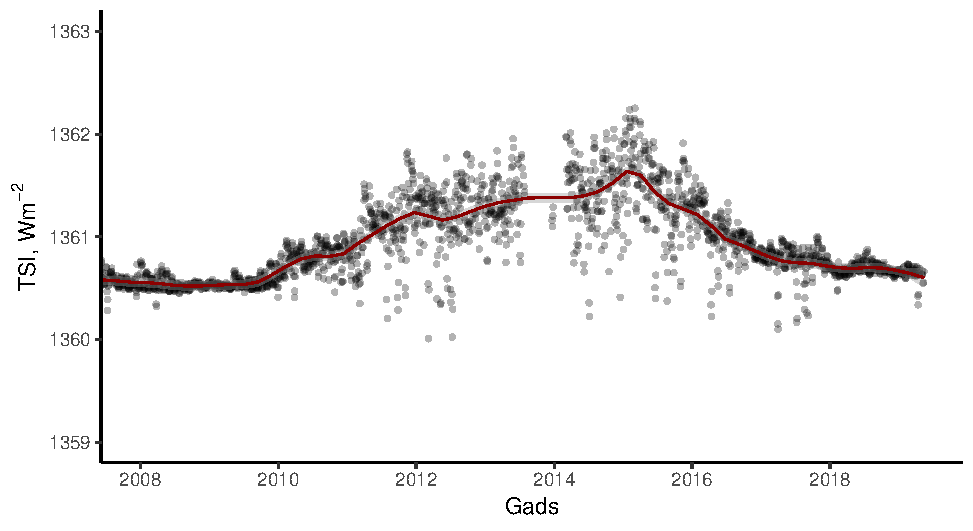
\includegraphics[width=\linewidth]{figures/misc/TSI_8-19.pdf}
    \caption{TSI 24. saules ciklā 1AU attālumā (24 h vidējā vērtība)\cite{TSIdata}}
    \label{fig:TSI1}
\end{figure}

\begin{figure}[h]
    \centering
    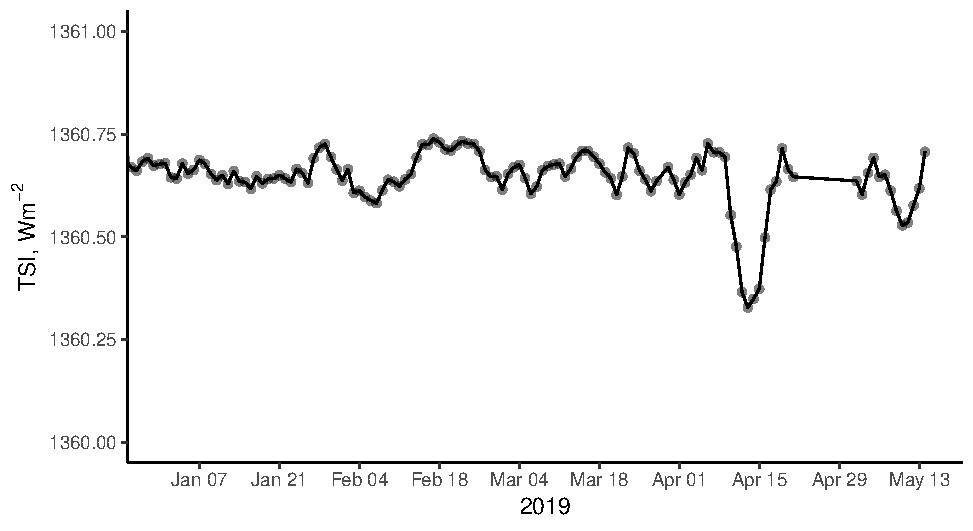
\includegraphics[width=\linewidth]{figures/misc/TSI.pdf}
    \caption{TSI izmaiņas solāro paneļu datu ieguves laikā 1AU attālumā (24 h vidējā vērtība)\cite{TSIdata}}
    \label{fig:TSI2}
\end{figure}

% \begin{figure}[h]
%     \centering
%     \includegraphics[width=\linewidth]{figures/misc/LV_DNI.png}
%     \caption{Tiešais normālais apstarojums \cite{solargis}}
%     \label{fig:lv_DNI}
% \end{figure}
% \begin{figure}[h]
%     \centering
%     \includegraphics[width=\linewidth]{figures/misc/LV_GHI.png}
%     \caption{Globālais horizontālais apstarojums Latvijā \cite{solargis}}
%     \label{fig:lv_GHI}
% \end{figure}
% \begin{figure}[h]
%     \centering
%     \includegraphics[width=\linewidth]{figures/misc/LV_PVOUT.png}
%     \caption{PV potenciālā jauda \cite{solargis}}
%     \label{fig:lv_PVOUT}
% \end{figure}

% !TeX spellcheck = lv_LV
% intensity
% spectral distribution
% solar geometry
% saules stāvoklis debesīs
% un virziens, kurā stara starojums krīt uz dažādu virzienu un ēnojuma virsmām

\section{Saules diennakts kustība}

Ģeometriskās attiecības starp saules paneļa virsmas plakni un ienākošo Saules starojuma kūli jeb Saules pozīcija relatīvi pret šo plakni tiek aprakstīta ar vairākiem leņķiem. Ar $\theta$ apzīmēsim staru krišanas leņķi uz saules paneli, pieņemot saules paneli par nekustīgu plakni. Tad, pie nemainīgas starojuma intensitātes, paneļa saņemtā enerģija būs proporcionāla $\cos{\theta}$ (ja $\theta<90^\circ$) vai būs vienāda ar 0 (ja $\theta>90^\circ$, t.i., Saules stari krīt uz paneļa apakšējo virsmu) pēc formulas \ref{eq:apgaismojums}. Saules diennakts kustība, gadalaiku cikls, kā arī saules paneļa novietojums ir ievēroti izteiksmē, kas ļauj aprēķināt $\cos{\theta}$ \cite{ThermalProcesses}:

\begin{equation}
\label{eq:apgaismojums}
E = I \cdot cos(\theta)
\end{equation}

\begin{equation}
\label{eq:theta}
\begin{aligned}
	\cos{\theta} = {} & \sin{\delta} \sin{\phi} \cos{\beta} - \sin{\delta} \cos{\phi} \sin{\beta} \cos{\gamma} +                           \\
	                  & \cos{\delta} \cos{\phi} \cos{\beta} \cos{\omega} + \cos{\delta} \sin{\phi} \sin{\beta} \cos{\gamma} \cos{\omega} + \\
	                  & \cos{\delta} \sin{\beta} \sin{\gamma} \sin{\omega},
\end{aligned}
\end{equation}
kur lietoti leņķi, kas definēti \ref{tab:theta} tabulā. Saules deklināciju solārajā pusdienlaikā var aprēķināt pēc formulas
\begin{equation}
\label{eq:delta}
    \delta = 23 \sin \left( 360 \cdot \frac{284+n}{365} \right),
\end{equation}
kur $n$ ir dienas kārtas numurs gadā.

Ar vienādojumu \ref{eq:theta} un \ref{eq:delta} palīdzību ir iespējams aprēķināt $\cos{\theta}$ laika atkarības, kas ir pirmais tuvinājums Saules apstarojuma izmaiņām dienas laikā.
Parametru vērtības katram no darbā lietotajiem Saules paneļiem ir apkopotas \ref{tab:param}. tabulā.
Lietojot šos parametrus, tika aprēķinātas $\cos{\theta}$ atkarības no laika diviem datumiem: 1. janvārim un 30. aprīlim (skat. \ref{fig:cos-theta}. att.). No tā secināms, ka austrumu virzienā uzstādītais panelis saņem vairāk apstarojuma no rīta nekā rietumu virzienā vērstais panelis. Pēc šī aprēķina iespējams prognozēt paneļu saražotās enerģijas izmaiņas gada griezumā, piemēram, no dienvidu paneļiem janvārī efektīvākais 90$^\circ$ leņķī vērstais, jo Saule atrodas zemu pie horizonta, bet aprīlī efektīvākais ir 40$^\circ$ leņķi.

\begin{table}[h!]
	\caption{Leņķu, kas lietoti \ref{eq:theta} vienādojumā, definīcijas.}
	\begin{center}
		\begin{tabular}{|c|c|l|}
			\hline
			         &         apgabals         & definīcija                                                                 \\ \hline
			$\theta$ &  $(0^\circ;180^\circ)$   & staru krišanas leņķis uz Saules paneli                                     \\ \hline
			$\delta$ &  $(-23^\circ;23^\circ)$  & Saules deklinācija --- leņķis starp virzieniem uz Sauli un uz debess       \\
			         &                          & ekvatoru solārajā pusdienlaikā, pozitīvs Z virzienā                        \\ \hline
			 $\phi$  &  $(-90^\circ;90^\circ)$  & ģeogrāfiskais platums, pozitīvs Z virzienā                                 \\ \hline
			$\beta$  &  $(0^\circ;180^\circ)$   & paneļa slīpums --- leņķis starp Saules paneļa virsmu un horizontāli        \\ \hline
			$\gamma$ & $(-180^\circ;180^\circ)$ & paneļa azimuts --- leņķis starp virsmas normāles projekciju uz horizontālu \\
			         &                          & plakni un D virzienu, negatīvs A virzienā                                  \\ \hline
			$\omega$ & $(-180^\circ;180^\circ)$ & solārais stundu leņķis --- leņķis starp Saules stara virziena projekciju   \\
			         &                          & uz horizontālu plakni un D virzienu (kas mainās Zemes rotācijas ap         \\
			         &                          & savu asi dēļ), negatīvs no rīta                                            \\ \hline
		\end{tabular}
	\end{center}
	\label{tab:theta}
\end{table}

\begin{table}[h!]
	\caption{Darbā lietotajiem Saules paneļiem atbilstošās leņķisko parametru vērtības, grādos.}
	\begin{center}
		\begin{tabular}{|r|c|c|c|c|c|}
			\hline
			         & R.13 & A.13 &   D.13   & D.40 & D.90 \\ \hline\hline
			paneļa slīpums $\beta$  & \multicolumn{3}{c|}{13} &  40  &  90  \\ \hline
			paneļa azimuts $\gamma$ &  90  & -90  & \multicolumn{3}{c|}{0}  \\ \hline
			ģeogrāfiskais platums $\phi$  &        \multicolumn{5}{c|}{57}        \\ \hline
		\end{tabular}
	\end{center}
	\label{tab:param}
\end{table}

\begin{figure}[h]
	\centering
	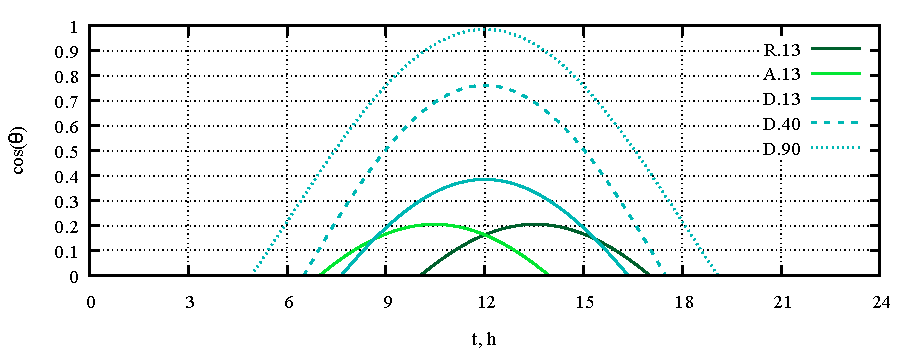
\includegraphics[width=\linewidth]{figures/misc/cos-theta-jan.pdf}
	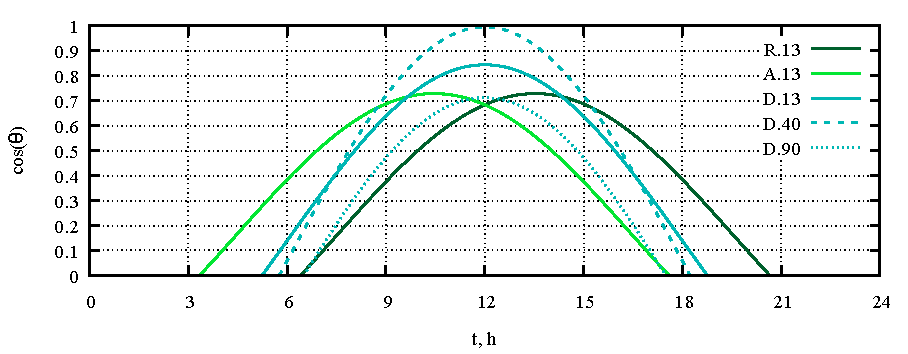
\includegraphics[width=\linewidth]{figures/misc/cos-theta-apr.pdf}
	\caption{Diennakts laikā paredzētas $\cos(\theta)$ vērtības darbā lietotajiem Saules paneļiem, aprēķinātas pēc \ref{eq:theta} izteiksmes 1. janvārim (augšā) un 30. aprīlim (apakšā).}
	\label{fig:cos-theta}
\end{figure}
\section{Klimats Latvijā}
%Enter antagonists. Mākoņi. Bloķē daudz saules apstarojuma. Cik LV mākoņainu dienu?
%Izanalizēt VTPMML meteo datus no 2013.
%Pajautāt Stasim kļūdas.

Tiek apskatīta atmosfēras un mākoņu ietekme uz virsmas saņemto saules starojumu, un tās praktiskā nozīme, apstrādājot pieejamos Saules starojuma datus.

Saskaņā ar LU VTPMML klimatisko datu apkopojumu, kas parādīts \ref{fig:makoni_Riga}. att., mākoņainība Rīgā var sasniegt līdz 60\% jūlijā un līdz pat 90\% decembrī. Tas nozīmē, ka Saules paneļu efektivitātes novērtējumam Latvijas klimatā mākoņainība ir ļoti būtiska un tā palīdzēs prognozēt nepieciešamos enerģijas uzkrājumus un papildavotus, ja solārā enerģija tiek izmantota kā pamata enerģijas avots.
\begin{figure}[h]
	\centering
	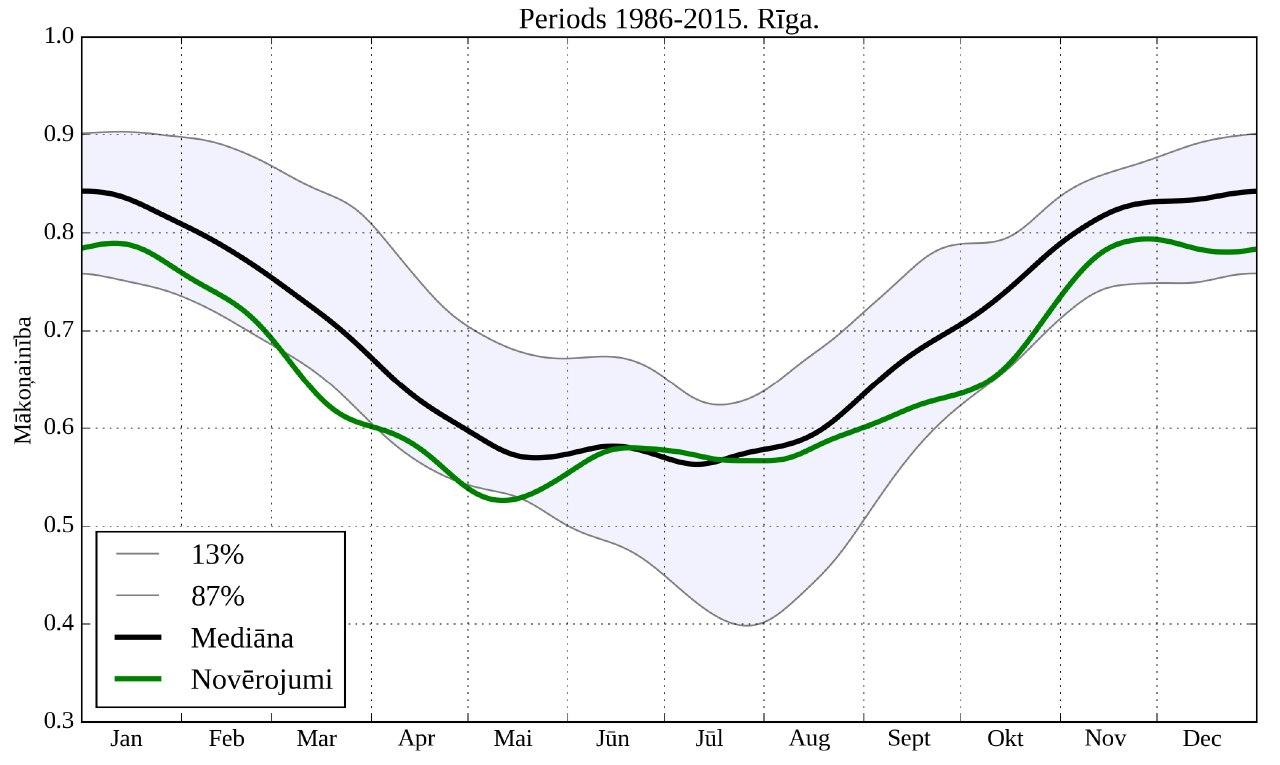
\includegraphics[width=0.8\linewidth]{figures/misc/makoni_riga.jpg}
	\caption{Vidējā mākoņainība Rīgā gada laikā, vidējota pa 20 gadu periodu~\cite{cloudsModlab}.}
	\label{fig:makoni_Riga}
\end{figure}

Mākoņu ietekme uz Saules apstarojumu ir komplicēta un atkarīga no dažādiem parametriem. Piemēram, pētījumā \cite{CloudCoverageImpactOnIrradiance} tiek parādīts, ka dažreiz mākoņainība var pat nedaudz palielināt Saules apstarojumu. Šis šķietami kontraintuitīvais rezultāts izskaidrojams ar to, ka Saule nav nosegta pilnībā, un baltie mākoņi mēdz būt gaišāki nekā pašas debesis saulainā dienā (skat. \ref{fig:makoni_ietekme}.(b) attēlā), tādējādi DNI komponentes samazināšanās tiek kompensēta ar palielinātu gaismas izkliedi. 

Savukārt gadījumos, kad mākoņi aizsedz Sauli (skat. \ref{fig:makoni_ietekme}.(c) attēlā), apstarojums $\approx99\%$ gadījumu samazinās, kā tas bija paredzams.
% Tomēr korelācija starp iegūto enerģiju un mākoņu daudzumu ir pat nedaudz pozitīva, kas atkal notiek palielinātas gaismas izkliedes dēļ. 
Apskatot visu datu kopu, var secināt, ka vairākumā gadījumu mākoņu ietekmi uz Saules paneļu saražoto enerģiju var uzskatīt par nelabvēlīgu.
Pētījumi rāda, ka mākoņi absorbē par 25 W/m$^2$ vairāk gaismas, nekā teorētiski paredzams, un šī vērtība nevar būt izskaidrojama ar troposfēras aerosoliem ~\cite{observVSModel}. Neskatoties uz to, ka mākoņainība ir galvenais Saules paneļu efektivitāti ietekmējošs faktors, ar informāciju par mākoņainību nepietiek, lai pilnvērtīgi izskaidrotu un paredzētu paneļu saražotās enerģijas izmaiņas.

\begin{figure}[h]
	\centering
	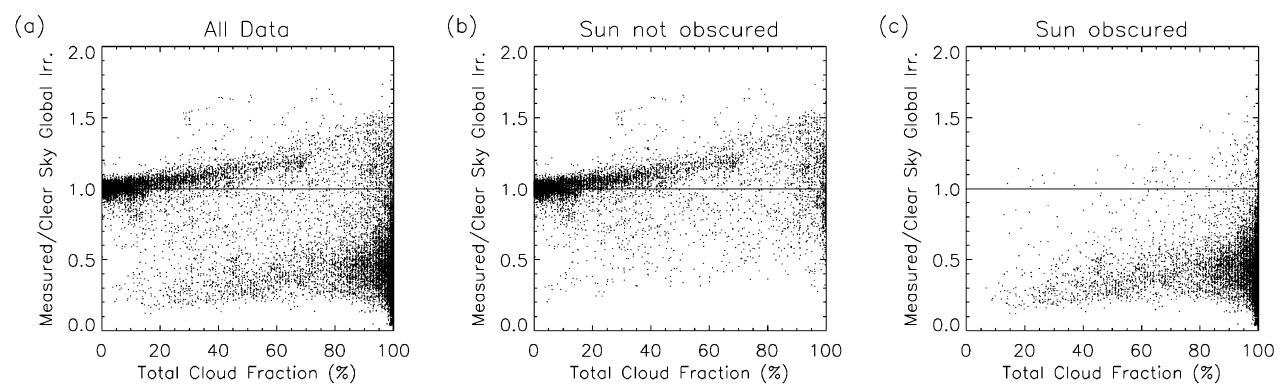
\includegraphics[width=\linewidth]{figures/misc/makoni_ietekme.jpg}
	\caption{Attiecība starp izmērīto apstarojumu un tīrās debess gadījuma apstarojumu (a) visiem datiem, (b) gadījumos ar neaizsegtu Sauli un (c) gadījumos ar aizsegtu Sauli~\cite{CloudCoverageImpactOnIrradiance}.}
	\label{fig:makoni_ietekme}
\end{figure}

Mākoņu ietekme ir atkarīga arī no to veida. Mākoņu modifikācijas reizinātājs (\textit{Cloud Modification Factor} - CMF), ko definē kā attiecību starp apstarojumu gadījumos ar un bez mākoņiem, atkarībā no mākoņu tipa ir apkopots \ref{tab:CMF}. tabulā. Ir jāņem vērā, ka CMF ir atkarīgs no viļņa garuma. Tomēr ultravioletais CMF no redzamās gaismas CMF ir atkarīgs lineāri ar koeficientiem $\approx0.6-1$ gubumākoņu gadījumā un eksponenciāli spalvmākoņu gadījumā.
\begin{table}[h]
	\caption{CMF intervāls atkarībā no mākoņu tipa~\cite{effectCloudsOnSurface}}
	\begin{center}
		\begin{tabular}{| r | c |}
			\hline
			augstie gubumākoņi & $<0.7$     \\ \hline
			gubumākoņi         & $0.2-1.3$ \\ \hline
			spalvmākoņi        & $0.6-1$    \\ \hline
		\end{tabular}
	\end{center}
	\label{tab:CMF}
\end{table}

Modelēt saules apstarojumu, kas nonāk paneļu virsmas, laikā komplicē ne tikai mākoņu ietekme, bet arī Saules apstarojuma izmaiņas laikā. Tomēr šī darba ietvaros to var neņemt vērā, jo globālais horizontālais apstarojums (GHI) mainās tikai ap 0.7~W/m$^2$ gadā. Atsaucoties uz TIM satelīta izmērīto saules gaismā ietverto enerģiju (skat.~\ref{fig:SSI}. att.), šis grafiks (skat.~\ref{fig:zudumi}. att.) attēlo enerģijas zudumus dažādiem viļņu garumiem absorbējoties atmosfērā, kā arī siltuma un sprieguma zudumus saules šūnā.

\begin{figure}[h]
    \centering
    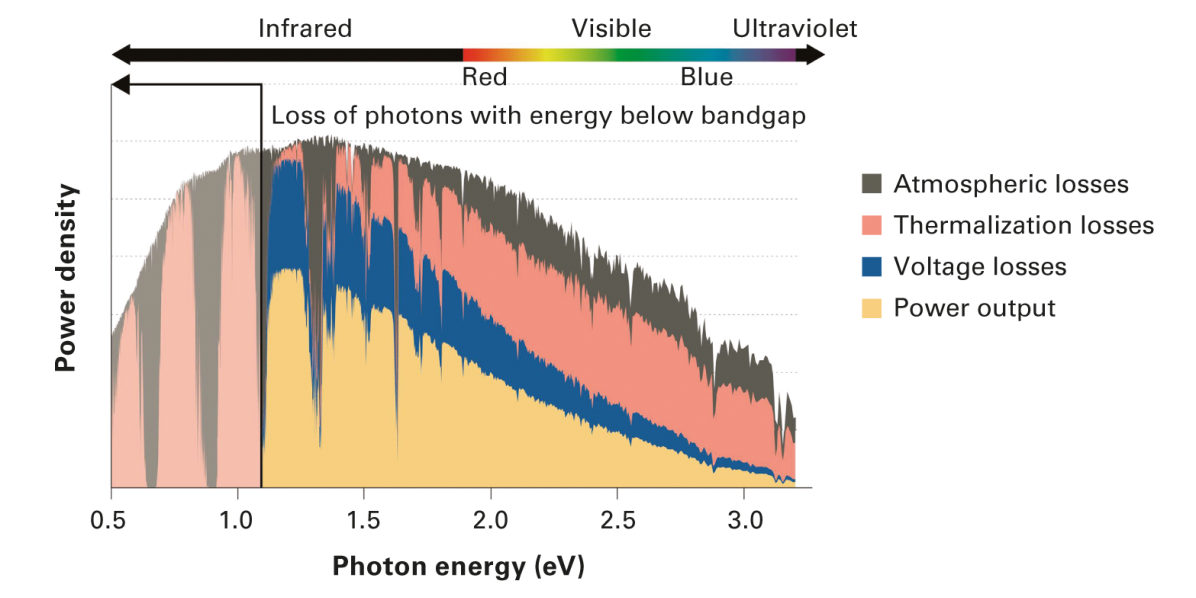
\includegraphics[width=\linewidth]{figures/misc/energyLosses.png}
    \caption{Saules enerģijas zudumi silīcijā balstītā saules šūnā (a) atmosfēras, (b) siltuma, (c) sprieguma, kā arī (d) producētā jauda  ~\cite{Sivaram}.}
    \label{fig:zudumi}
\end{figure}

% DNI vidēji 1025 kWh/m2
% GHI vidēji arī bet vairāk

Pēc Solargis modeļa no satelītu un atmosfēras mērījumu datiem ar kļūdu 3\% līdz 10\% robežās secināms, ka piekrastē ir vairāk saules apstarojuma un līdz ar to arī lielāka prognozētā jauda. 
Tiešais normālais apstarojums (\textit{Direct normal irradiance} - DNI) ir Saules apstarojums bez izkliedes atmosfērā
Globālais horizontālais apstarojums (\textit{Global horizontal irradiance} - GHI) ir kopējais virsmas saņemtais apstarojums, ieskaitot gan DNI, gan starojumu, kas izkliedējas atmosfērā.

Salīdzinot \ref{fig:lv_DNI}. un  \ref{fig:lv_DNI}. attēlus redzams, ka GHI ir nedaudz lielāks par DNI, tātad redzams izkliedētā starojuma ieguldījums. PVOUT karte sniedz apkopojumu par prognozēto saules fotoelementu (PV) enerģijas ražošanas apjomu, pieņemot 1kW jaudas silīcija PV spēkstacijas, gada patēriņam optimizētu slīpuma leņķi \ref{fig:lv_PVOUT}. Pēc šiem datiem kopumā var secināt, ka saules paneļi ir piemērots risinājums enerģijas ieguvei arī Latvijā.


\begin{figure}[h]
    \centering
    \includegraphics[width=0.8\linewidth]{figures/misc/LV_DNI.png}
    \caption{Tiešais normālais apstarojums Latvijā \cite{solargis}}
    \label{fig:lv_DNI}
\end{figure}
\begin{figure}[h]
    \centering
    \includegraphics[width=0.8\linewidth]{figures/misc/LV_GHI.png}
    \caption{Globālais horizontālais apstarojums Latvijā \cite{solargis}}
    \label{fig:lv_GHI}
\end{figure}
\begin{figure}[h]
    \centering
    \includegraphics[width=0.8\linewidth]{figures/misc/LV_PVOUT.png}
    \caption{PV potenciālā jauda Latvijā \cite{solargis}}
    \label{fig:lv_PVOUT}
\end{figure}
\section{Saules paneļi}
% KĀ STRĀDĀ SAULES PANEĻI?
% fotons uzspīd elektronam un viņu ierosina un tad tas aiziet pāri vadītspējas zonai un aizpeld uz elektrodu un caurums aizpeld uz otru elektrodu un rodas potenciālu starpība no kurienes strāva.
% Ielikt dokus par LG un JA tipu + no kādiem kristāliem tie
% Ielikt shēmu
% analīze par saules paneļu plantācijām pasaulē
% optimālie apstākļi?

Saules paneļi sastāv no fotoelementiem, kas pārveido gaismas enerģiju elektriskajā enerģijā. Fotoelements, kura uzbūves shēma ir parādīta \ref{fig:PV}. attēlā, ir p-n pāreja ar elektriskiem kontaktiem, kas pieslēgti pie lādētāja vai citas enerģijas patērētāja. Fotoelementa apakšējā daļa sastāv no n-tipa pusvadītāja, kurā lādiņa pamatnesēji ir elektroni, bet augšējā daļa --- no p-tipa pusvadītāja, kur lādiņa pamatnesēji ir caurumi. 

Fotoelementa darbība balstās uz iekšējo fotoelektrisko efektu --- parādību, kad elektrons tiek ierosināts ar gaismas kvantu un pāriet no valences zonas uz vadītspējas zonu. Kad tas notiek augšējā slānī (p-tipa pusvadītājā), elektrons atgrūžas no robežas starp slāņiem, kura ir negatīvi lādēta rekombinācijas dēļ. Negatīvi lādētā (no p-tipa pusvadītāja puses) robeža rada potenciālu starpību, kas veicina elektronu kustību pa vadiem uz patērētāju, tādā veidā radot elektrisko strāvu.

\begin{figure}[h]
    \centering
    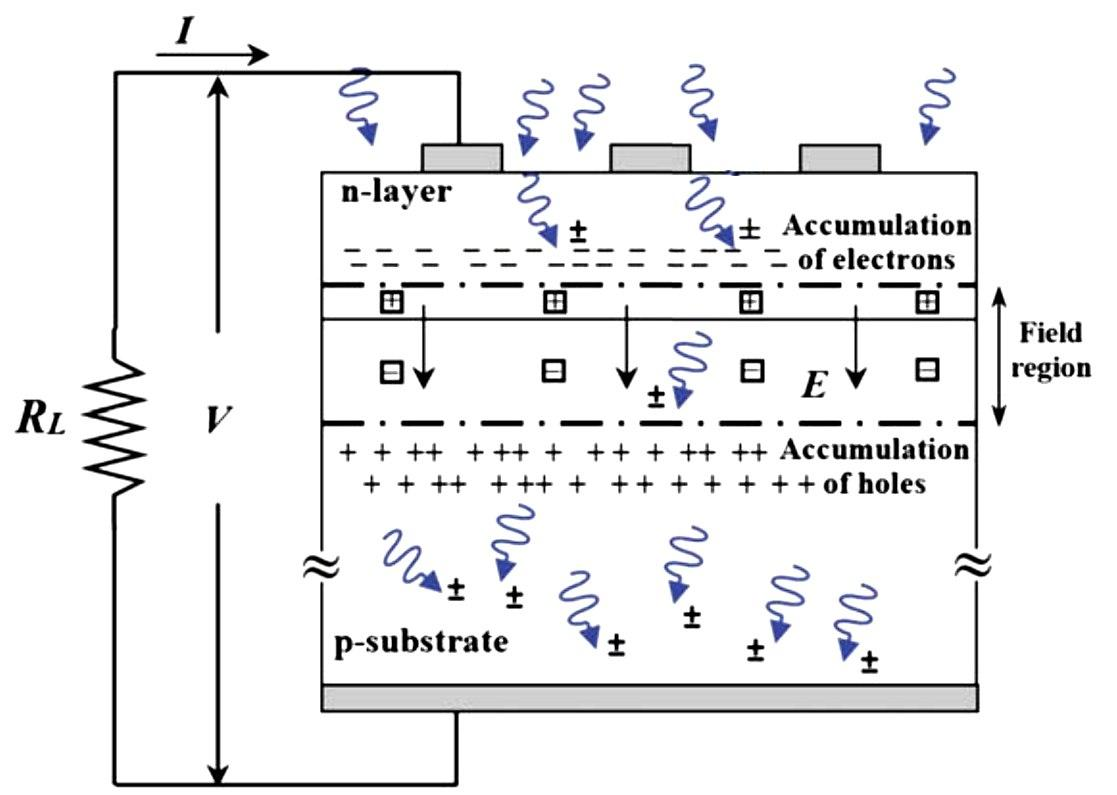
\includegraphics[width=0.6\linewidth]{figures/misc/PV.jpg}
    \caption{Saules paneļa shēma. Tas sastāv no fotoelementiem, kuru augšējais slānis veidots no p-tipa pusvadītāja, bet apakšējais --- no n-tipa pusvadītāja.}
    \label{fig:PV}
\end{figure}

P-tipa un n-tipa pusvadītāja īpašības var panākt, piemēram, dopējot silīcija kristālu ar attiecīgi III vai V grupas elementiem. Ja silīcija kristālam pievieno bora atomus nelielā koncentrācijā, izveidojas \ref{fig:p-n-type}. att. pa kreisi redzamā situācija. Katram Si atomam ir četri elektroni ārējā čaulā, ar kuru palīdzību atoms izveido četras kovalentās saites ar četriem citiem atomiem. Savukārt bors, būdams III grupas elements, var izveidot tikai trīs saites. Tādā veidā pie bora atoma parādās "caurums" --- nenoslēgta kovalentā saite, kas attēlā apzīmēta ar sarkanu līniju. Uz šo vietu var pārvietoties kāds no blakus esošiem elektroniem, bet tad neaizpildīta vieta parādīsies pie blakus esošā atoma. Tādā veidā var uzskatīt, ka caurums pārvietojas, un nosaukt to par pozitīvo lādiņa nesēju. Šādus pusvadītājus sauc par p-tipa pusvadītājiem.

Ja silīcija kristālam pievieno fosfora atomus, izveidojas pretēja situācija --- pie P atoma parādās elektrons, kas nepiedalās saites veidošanā (sk. att. \ref{fig:p-n-type}., pa labi). Lai pārvietotos, brīvajam elektronam ir nepieciešams mazāk enerģijas nekā elektroniem, kas veido kovalentās saites starp Si atomiem. Tātad, lādiņa pamatnesēji n-tipa pusvadītājos ir elektroni, un šādus pusvadītājus sauc par p-tipa pusvadītājiem.

Dopējot divus blakus esošus Si kristāla apgabalus dažādā veidā, iegūst p-n pāreju. Uz robežas starp apgabaliem elektroni no n-tipa apgabala var difūzijas ceļā nokļūt uz p-tipa apgabalu un aizpildīt tos caurumus, kas atrodas pietiekami tuvu. To sauc arī par elektronu-caurumu rekombināciju. Tādā veidā p-tipa pusvadītāja mala uzlādējās negatīvi. 

\begin{figure}[h]
	\centering
	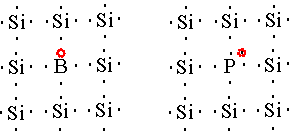
\includegraphics[width=0.5\linewidth]{figures/misc/p_n_type.pdf}
	\caption{Silīcija kristāla 2D izklājums, atomu ārējās čaulas elektroni ir apzīmēti ar punktiem. Pievienojot bora atomu, iegūst p-tipa pusvadītāju (pa kreisi), bet fosfora atomu --- n-tipa pusvadītāju (pa labi).}
	\label{fig:p-n-type}
\end{figure}


\subsection{Paneļu veidi}

Darbā ir apskatīti divi Saules paneļu veidi:
\begin{itemize}
	\item LG
	\item JA
\end{itemize}

%* Rezultāti
\chapter{Rezultāti un diskusija}
\input{tex/rezultati}
\section{Saules apstarojums}
% \begin{figure}[h]
%     \centering
%     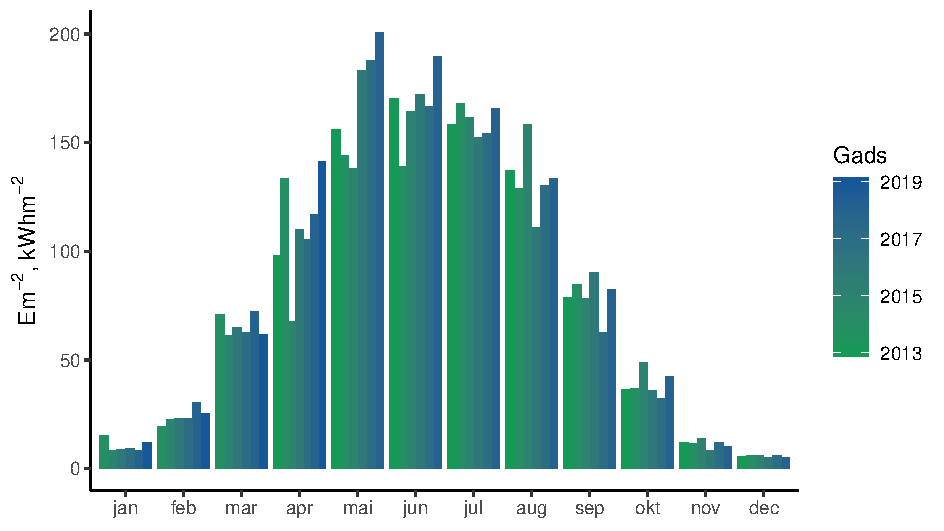
\includegraphics[width=\linewidth]{figures/meteo/statsYears.pdf}
%     \caption{Solārā apstarojuma laika integrāļa atšķirības gada gaitā. Eksperimentālā poligona meteostacijas stacijas dati 2013 -- 2019 periodā.}
%     \label{fig:metYears}
% \end{figure}

% izlabo visur lu meteoroloģiju uz poligonu
% pārsaukt grafikā Em^-2 uz E_{norm} (normētais enerģijas blīvums)

\begin{figure}[h]
    \centering
    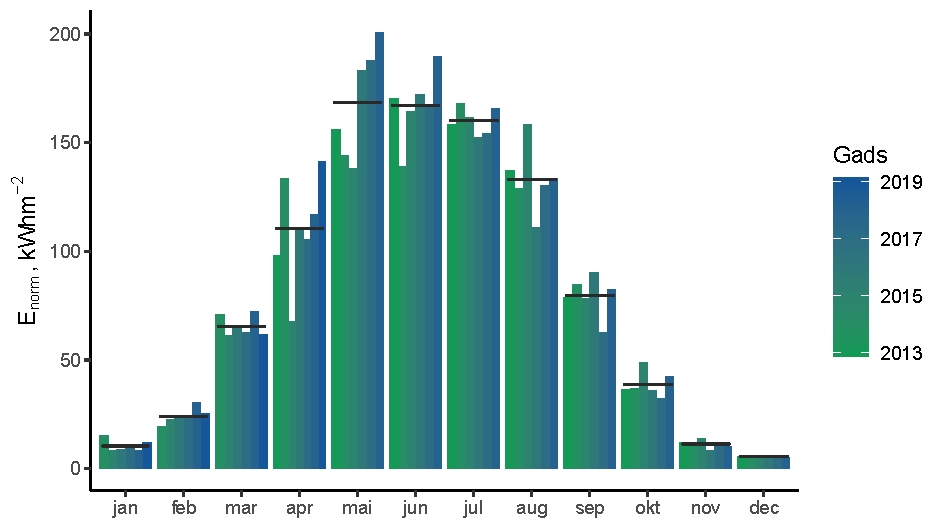
\includegraphics[width=\linewidth]{figures/meteo/meanYears.pdf}
    \caption{Solārā apstarojuma laika integrāļa atšķirības gada gaitā un to vidējās vērtības. Eksperimentālā poligona meteostacijas stacijas dati 2013 -- 2019 periodā.}
    \label{fig:metYears_mean}
\end{figure}
\begin{figure}[h]
    \centering
    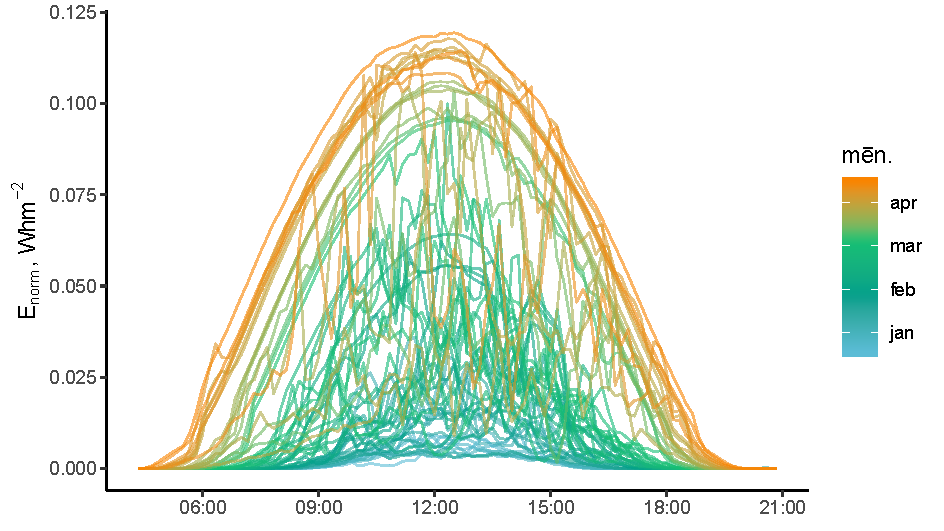
\includegraphics[width=\linewidth]{figures/meteo/sun19.pdf}
    \caption{Solārā apstarojuma izmaiņas dienas gaitā. Eksperimentālā poligona meteostacijas stacijas dati 2019-01-01 -- 2019-04-31 periodā.}
    \label{fig:met_Irrad}
\end{figure}
\begin{figure}[h]
    \centering
    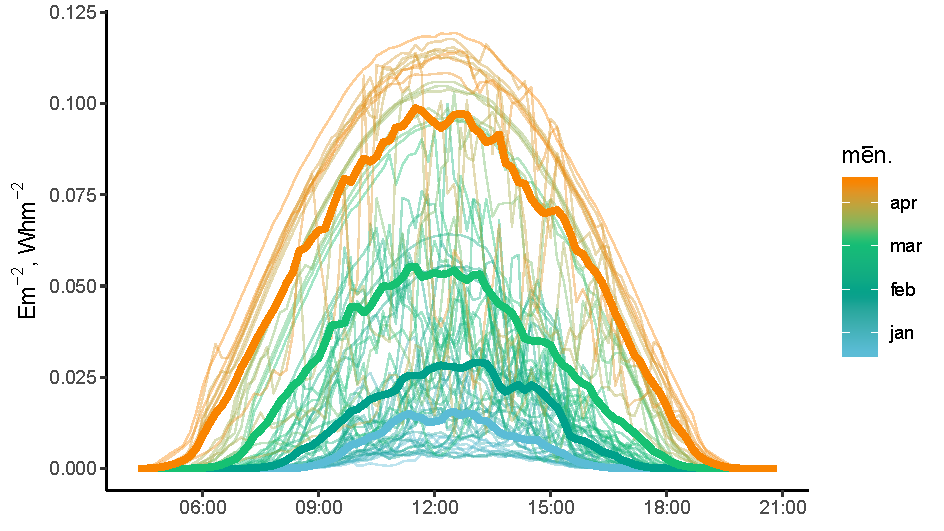
\includegraphics[width=\linewidth]{figures/meteo/mean19.pdf}
    \caption{Mēnesī vidējotas solārā apstarojuma izmaiņas dienas gaitā. Eksperimentālā poligona meteostacijas stacijas dati 2019-01-01 -- 2019-04-31 periodā.}
    \label{fig:met_Irrad_mean}
\end{figure}
\section{Efektivitātes atkarība no parametriem}
\subsection{Saules paneļa tipa} \label{subsection:tipi}

Pēc tabulām \ref{tab:JA} un \ref{tab:LG}, kā arī grafikiem, kas integrēti diskusijā par citu parametru ietekmi uz efektivitāti (skat. \ref{subsection:gads}. nod.), redzams, ka LG tipa paneļi konsekventi ir efektīvāki par JA tipu. Tas ir saistīts gan ar kristāla veidu -- kā pierādīts \ref{section:tipi}. nod.,  monokristāliska Si paneļi ir ražīgāki par polikristāliem --, gan paneļu maksimālajām jaudām -- LG tā ir lielāka nekā JA.

\begin{table}[h]
    \caption{JA tipa paneļu saražotā enerģija uz kvadrātmetru\\ salīdzināta ar piranometra izmērīto enerģiju}
    \begin{center}
    %%%%%%%%%%%%%%%%%%%%%%%%%%%%%%%%%%%%%%%%%%%%%%%%%%%%%%%%%%%%%%%%%%%%%%
%%                                                                  %%
%%  This is a LaTeX2e table fragment exported from Gnumeric.        %%
%%                                                                  %%
%%%%%%%%%%%%%%%%%%%%%%%%%%%%%%%%%%%%%%%%%%%%%%%%%%%%%%%%%%%%%%%%%%%%%%
\begin{tabular}{ | c | r r r r r  r | } \hline
E, $\textrm{kWhm}^{-2}$	&A.13	&R.13	&D.13	&D.40	&D.90	&piranometrs\\ \hline
jan		&0.35	&0.23	&0.72	&2.46	&2.80		&12.14\\
feb		&3.20	&2.74	&4.27	&6.45	&5.99		&25.14\\
mar		&8.22	&7.40	&9.47	&11.94	&8.72		&61.76\\
apr		&19.89	&19.23	&23.27	&25.43	&18.25		&141.41\\ \hline
$E_{sum}$, $\textrm{kWhm}^{-2}$
		&31.7	&29.6	&37.7	&46.3	&35.8 	&240.5\\ \hline
\end{tabular}
    \end{center} \label{tab:JA}
\end{table}
\begin{table}[h]
    \caption{LG tipa paneļu saražotā enerģija uz kvadrātmetru\\ salīdzināta ar piranometra izmērīto enerģiju}
    \begin{center}
    %%%%%%%%%%%%%%%%%%%%%%%%%%%%%%%%%%%%%%%%%%%%%%%%%%%%%%%%%%%%%%%%%%%%%%
%%                                                                  %%
%%  This is a LaTeX2e table fragment exported from Gnumeric.        %%
%%                                                                  %%
%%%%%%%%%%%%%%%%%%%%%%%%%%%%%%%%%%%%%%%%%%%%%%%%%%%%%%%%%%%%%%%%%%%%%%
\begin{tabular}{ | c | r r r r r  r | } \hline
E, $\textrm{kWhm}^{-2}$	&A.13	&R.13	&D.13	&D.40	&D.90 	&piranometrs\\ \hline
jan	&0.5	&0.35	&0.95	&2.82	&3.22		&12.14	\\
feb	&4.43	&3.63	&5.05	&8.25	&7.41		&25.14	\\
mar	&10.92	&9.27	&11.27	&15.69	&11.34		&61.76	\\
apr	&27.63	&25.46	&29.14	&34.21	&23.18		&141.41	\\ \hline
$E_{sum}$, $\textrm{kWhm}^{-2}$
	&43.48	&38.7	&46.41	&60.98	&45.14		&240.46	\\ \hline
\end{tabular}
    \end{center} \label{tab:LG}
\end{table}

% %%%%%%%%%
\subsection{Saules paneļa leņķa}\label{subsection:degree}
Apkopojot četru mēnešu datus un abus paneļu tipus, visražīgākais leņķis ir 40\textdegree.
Kopumā var secināt, ka paneļi 90\textdegree ~leņķī ir saražo vairāk enerģijas ziemas mēnešos un 13\textdegree ~leņķī -- vasaras mēnešos, tātad apstrinās teorijā prognozētais (skat.\ref{section:kustiba}.nod).
% Tas sakrīt ar [ielikt grafiku ar LV karti un optimālo leņķi bet es neatceros no kurienes paņēmu to].
\begin{figure}[h]
    \centering
    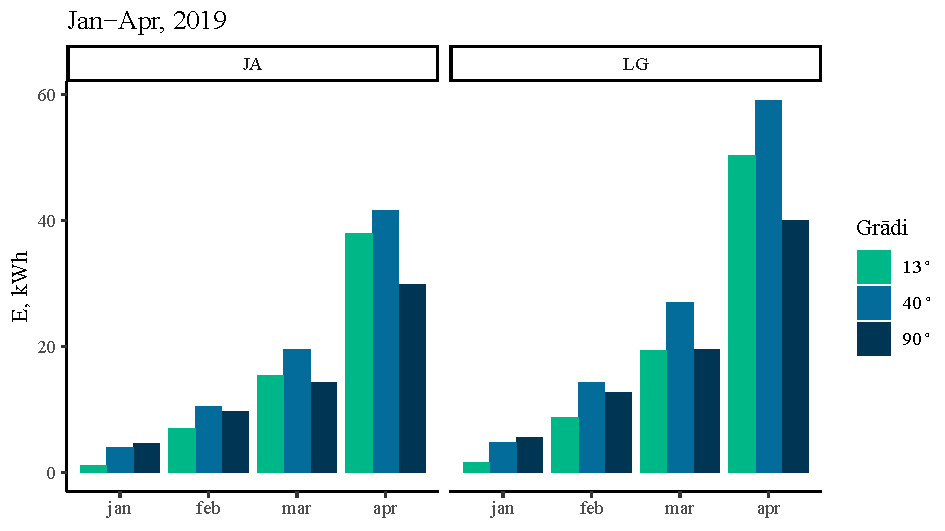
\includegraphics[width=\linewidth]{figures/results/all_degType.pdf}
    \caption{D virzienā vērsto saules paneļu saražotā enerģija atkarībā no leņķa un saules paneļu tipa} \label{fig:lg_ja_deg}
\end{figure}


\subsection{Saules paneļa virziena}\label{subsection:dir}
Visražīgākais virziens ir D, tad A, tad R. To paskaidro \ref{subsection:month_day}. nod. redzamie paneļu saražotās enerģijas dienas sadalījumi.
% no idea why tho
\begin{figure}[h]
    \centering
    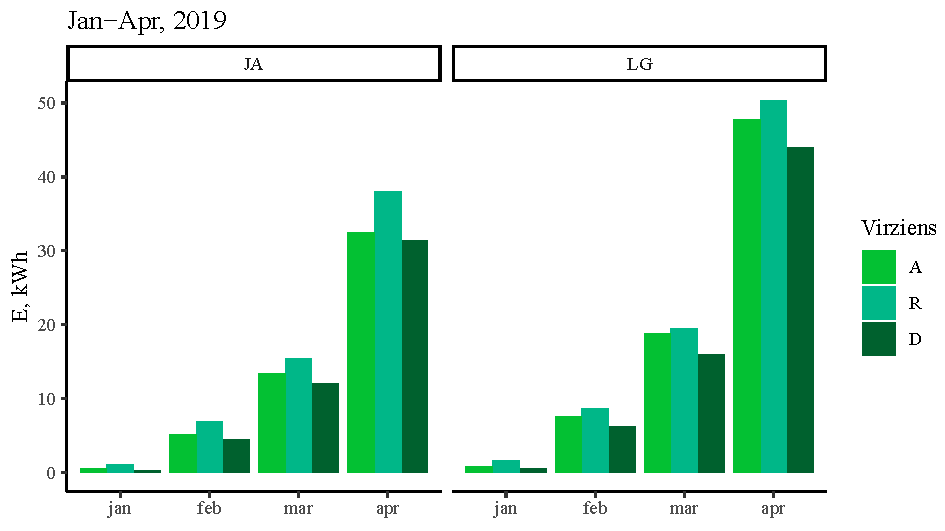
\includegraphics[width=\linewidth]{figures/results/all_dirType.pdf}
    \caption{13 grādu leņķī vērsto saules paneļu atkarība no virziena un saules paneļu tipa}
    \label{fig:lg_ja_dir}
\end{figure}

\subsection{Saules paneļa leņķa un virziena kombinācijas}
\label{subsection:month_day}

Saules paneļu saņemtā apstarojuma dienas sadalījuma tendenci drīkst salīdzināt ar attiecīgo paneļu saražotās enerģijas tendenci, jo pēdējā ir atkarīga no paneļa virsmas saņemtā Saules apstarojuma, kas savukārt ir funkcija no $cos(\theta)$, tātad proporcionāla tam. Salīdzinot \ref{fig:cos-theta}.(c) ar 
\ref{fig:toldU}, tiek secināts, ka eksperimentālie rezultāti sakrīt ar teoriju.

\begin{figure}[h]
    \centering
    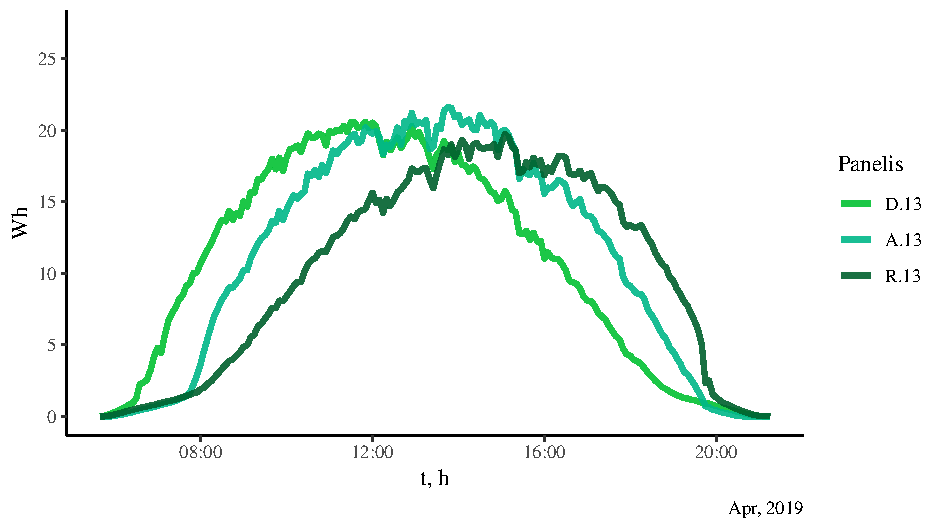
\includegraphics[width=\linewidth]{figures/sol_day/apr_LG_13.pdf}
    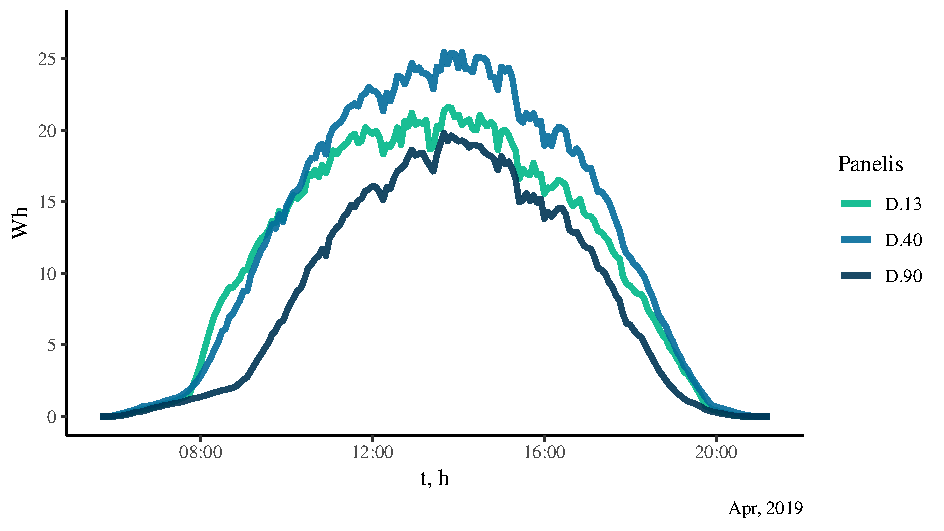
\includegraphics[width=\linewidth]{figures/sol_day/apr_LG_D.pdf}
    \caption{Saules paneļu saražotās enerģijas dienas sadalījuma līkne vidējotiem 27-30. aprīļa datiem} \label{fig:toldU}
\end{figure}

% \begin{figure}[h]
%     \centering
%     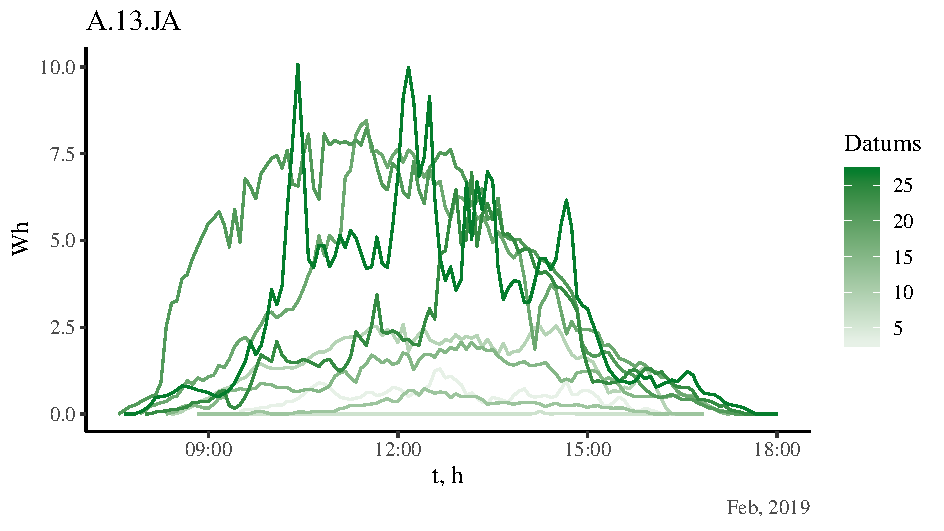
\includegraphics[width=\linewidth]{figures/sol_day/feb_A13JA.pdf}
%     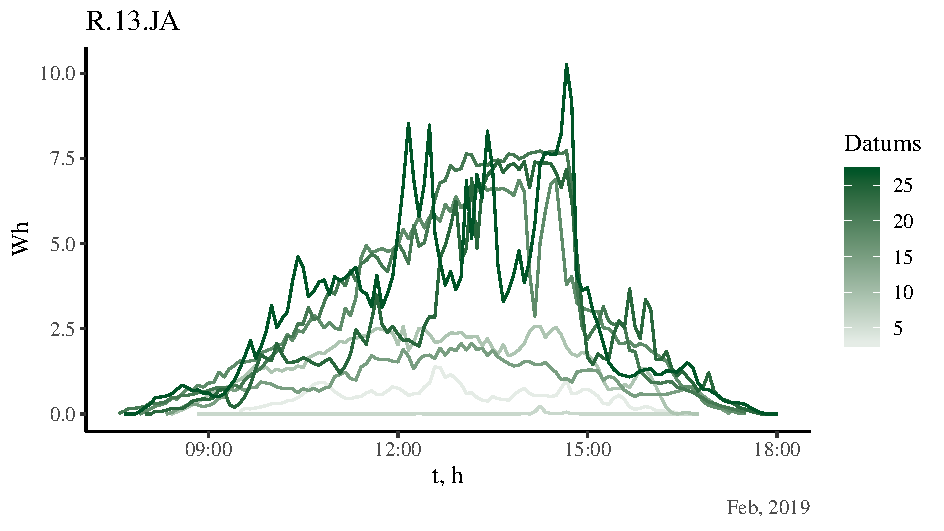
\includegraphics[width=\linewidth]{figures/sol_day/feb_R13JA.pdf}
%     \caption{A un R virzienu saules paneļu 5 minūtēs vidējotu Wh dienas sadalījumi februārī}
%     \label{fig:feb_ar}
% \end{figure}

% Kā redzams \ref{fig:feb_ar}, \ref{fig:mar_ar}, \ref{fig:apr_ar}. att., eksperimentāli noteiktais dienas sadalījums sakrīt ar teorētiski prognozēto \ref{fig:cos-theta}.att.
% \begin{figure}[h]
%     \centering
%     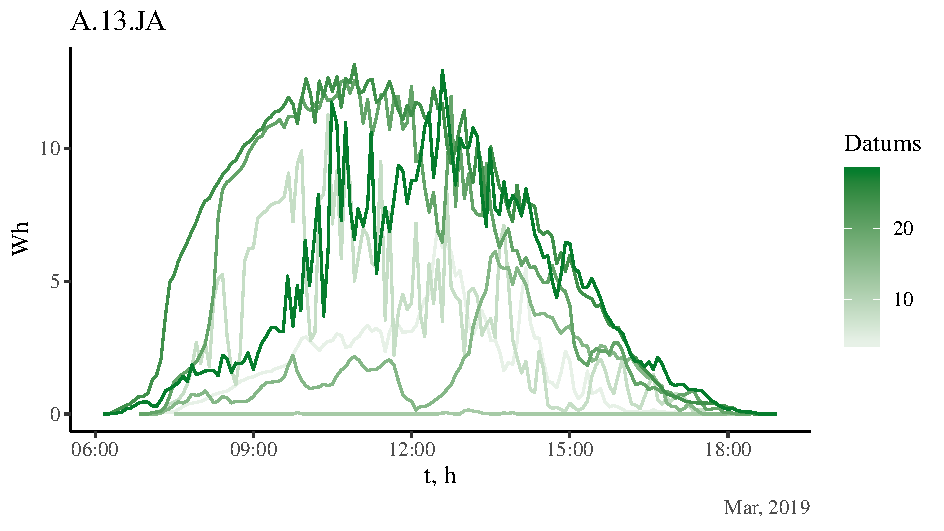
\includegraphics[width=\linewidth]{figures/sol_day/mar_A13JA.pdf}
%     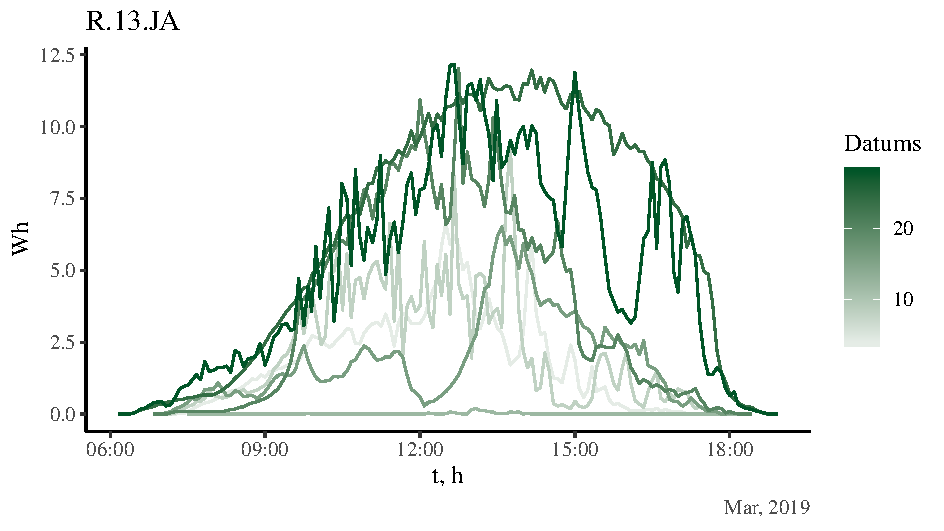
\includegraphics[width=\linewidth]{figures/sol_day/mar_R13JA.pdf}
%     \caption{A un R virzienu saules paneļu 5 minūtēs vidējotu Wh dienas sadalījumi martā}
%     \label{fig:mar_ar}
% \end{figure}

% \begin{figure}[h]
%     \centering
%     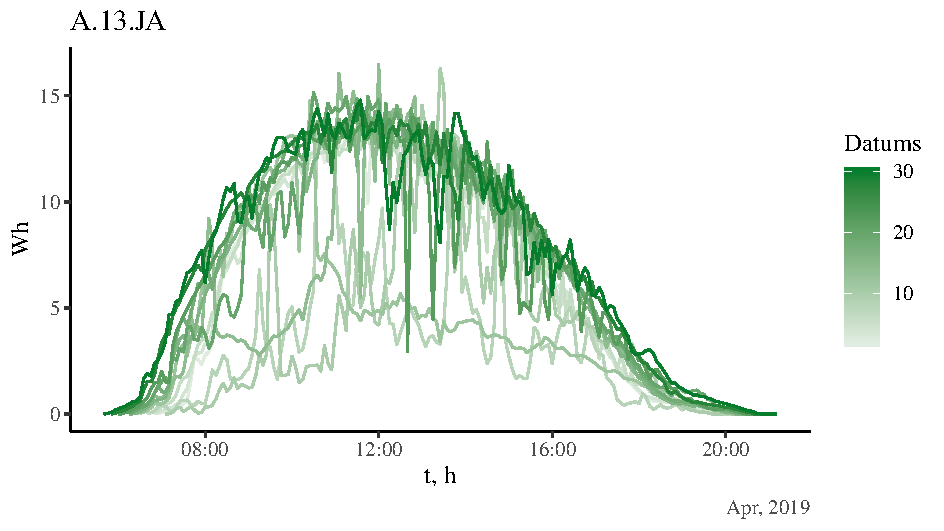
\includegraphics[width=\linewidth]{figures/sol_day/apr_A13JA.pdf}
%     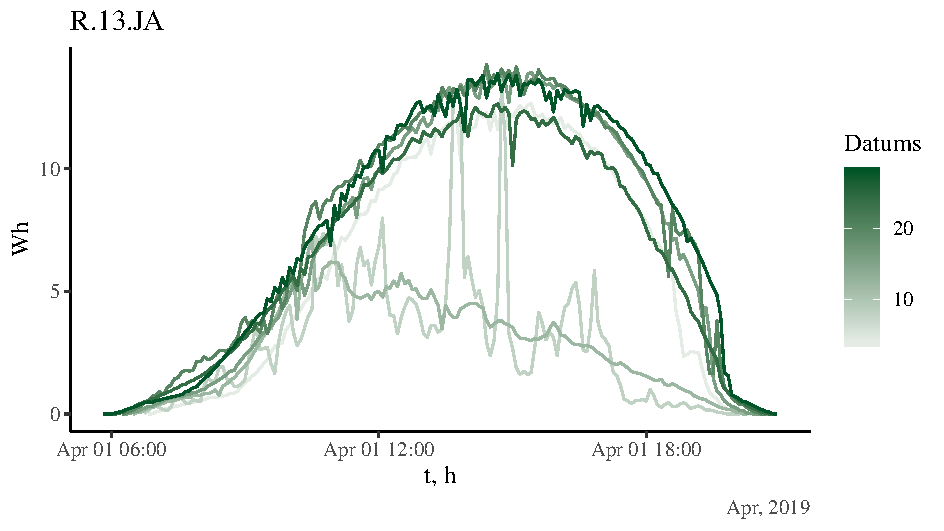
\includegraphics[width=\linewidth]{figures/sol_day/apr_R13JA.pdf}
%     \caption{A un R virzienu saules paneļu 5 minūtēs vidējotu Wh dienas sadalījumi aprīlī}
%     \label{fig:apr_ar}
% \end{figure}

% % \begin{figure}[h]
% %     \centering
% %     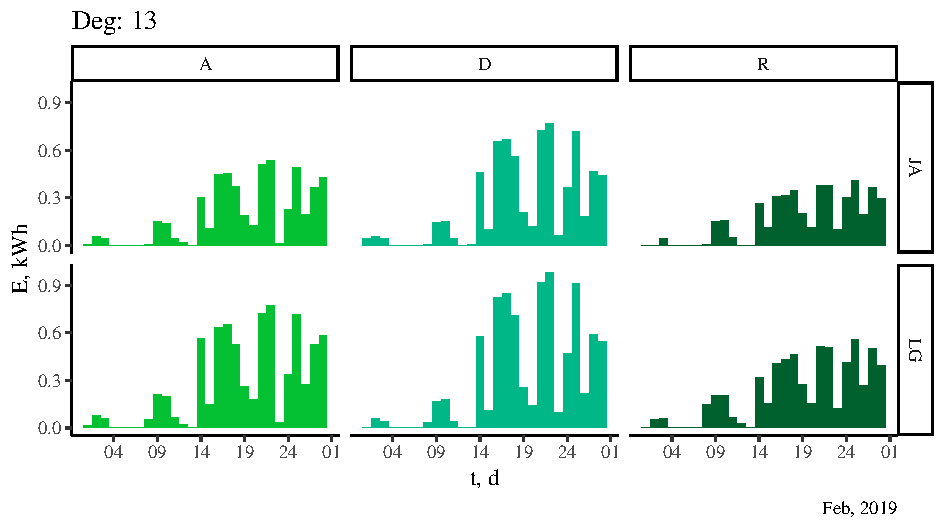
\includegraphics[width=\linewidth]{figures/sol_month/feb_Dir_d.pdf}
% %     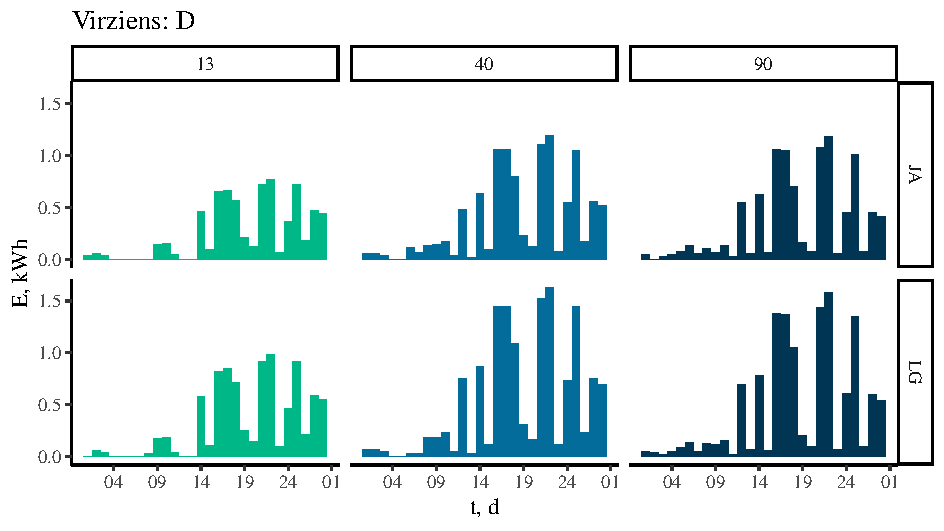
\includegraphics[width=\linewidth]{figures/sol_month/feb_Deg_d.pdf}
% %     \caption{Saules paneļu saražotā enerģija atkarībā no virziena un leņķa februārī}
% %     \label{fig:feb_degDir}
% % \end{figure}

% % \begin{figure}[h]
% %     \centering
% %     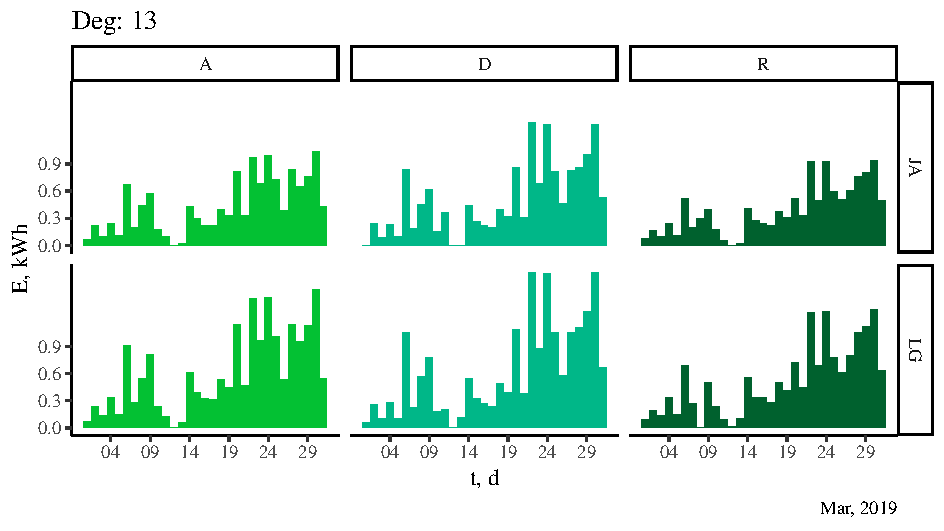
\includegraphics[width=\linewidth]{figures/sol_month/mar_Dir_d.pdf}
% %     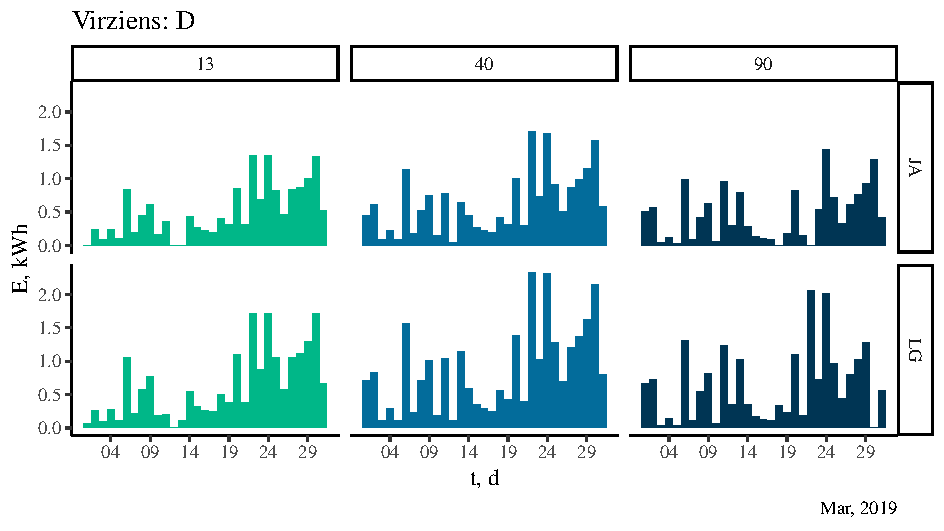
\includegraphics[width=\linewidth]{figures/sol_month/mar_Deg_d.pdf}
% %     \caption{Saules paneļu saražotā enerģija atkarībā no virziena un leņķa martā}
% %     \label{fig:mar_degDir}
% % \end{figure}

% % \begin{figure}[h]
% %     \centering
% %     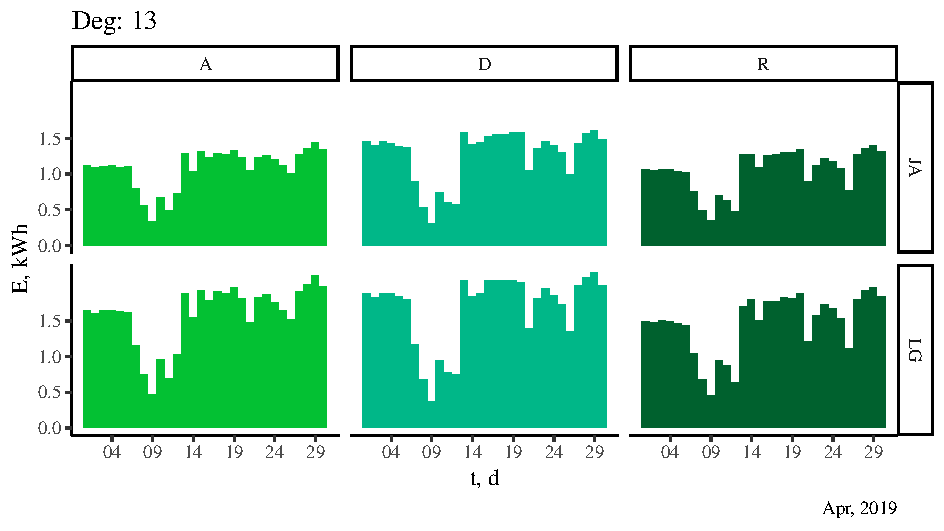
\includegraphics[width=\linewidth]{figures/sol_month/apr_Dir_d.pdf}
% %     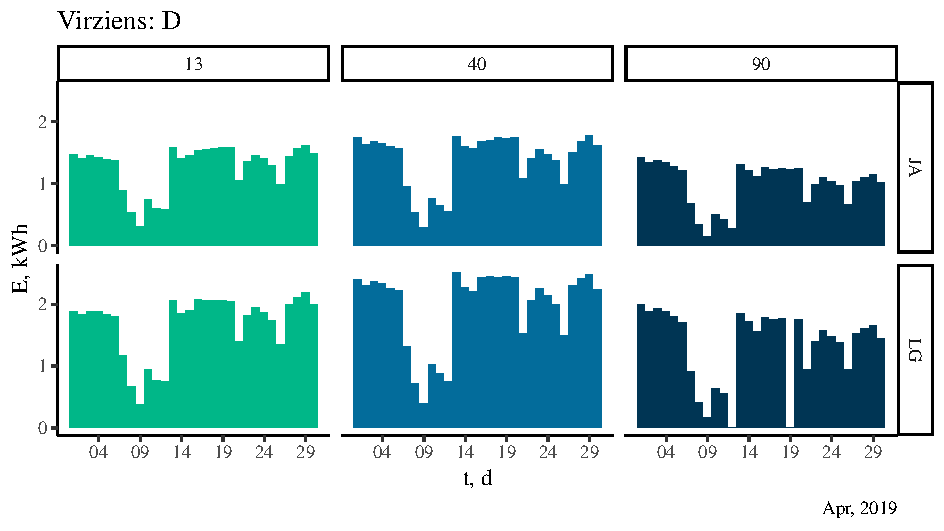
\includegraphics[width=\linewidth]{figures/sol_month/apr_Deg_d.pdf}
% %     \caption{Saules paneļu saražotā enerģija atkarībā no virziena un leņķa aprīlī}
% %     \label{fig:apr_degDir}
% % \end{figure}

\subsection{Gada mēneša} \label{subsection:gads}
Pēc \ref{fig:jan_sum}, \ref{fig:feb_sun}, \ref{fig:apr_sum}, \ref{fig:apr_sum}. att., tiek izdarīti secinājumi par saules paneļu ražīguma atkarību no gada mēneša. Janvārī visražīgākais panelis ir D.90, otrs ražīgākais - D.40, kas atbilst janvārim raksturīgajai Saules diennakts kustībai -- zemu pie horzionta. \ref{fig:feb_sun}. att. redzams, ka februārī D.40 kļūst ražīgāks nekā D.90, tāpat redzams, ka mazāku leņķu paneļi -- R.13 un A.13 -- ir palielinājuši ražīgumu. Šī tendence turpinās arī marta un aprīļa mēnešos.

\begin{figure}[h]
    \centering
    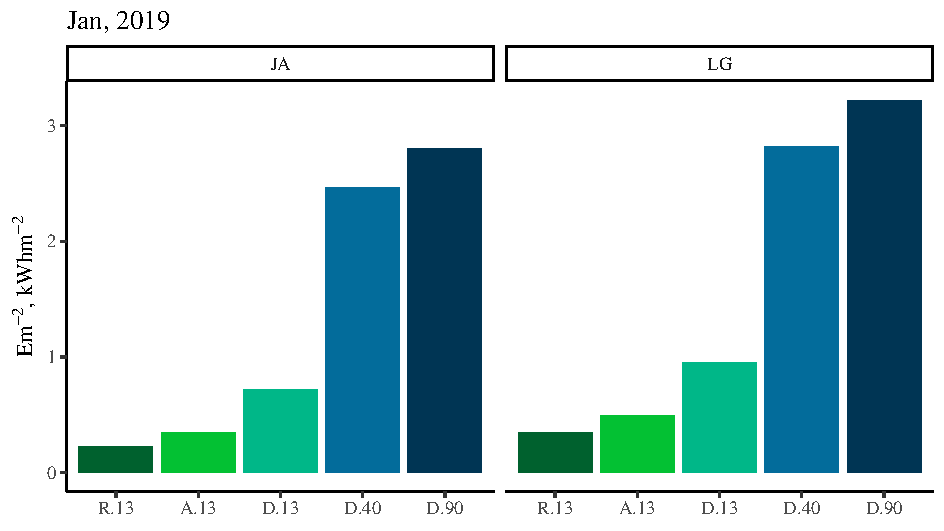
\includegraphics[width=\linewidth]{figures/sol_month/jan_m_m2.pdf}
    \caption{Saules paneļu saražotā enerģija janvārī}
    \label{fig:jan_sum}
\end{figure}

\begin{figure}[h]
    \centering
    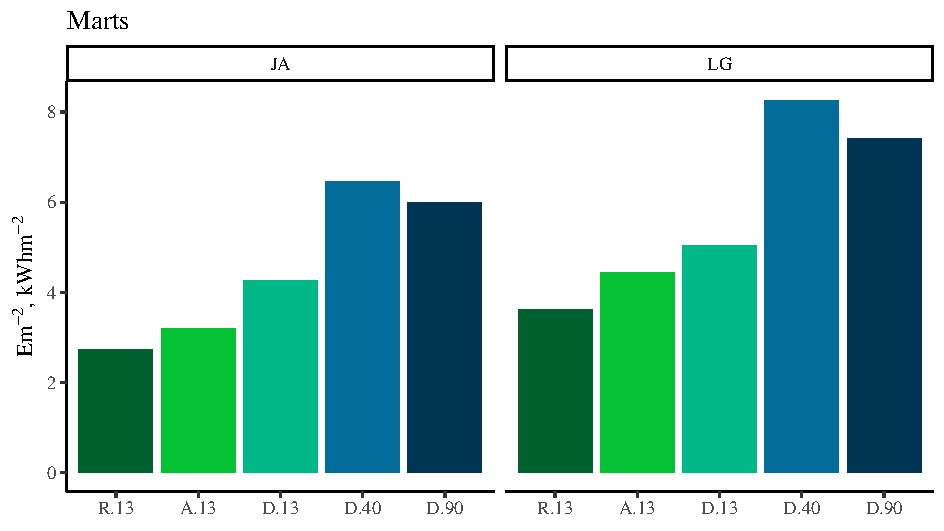
\includegraphics[width=\linewidth]{figures/sol_month/feb_m_m2.pdf}
    \caption{Saules paneļu saražotā enerģija februārī}
    \label{fig:feb_sum}
\end{figure}

% \begin{figure}[h]
%     \centering
%     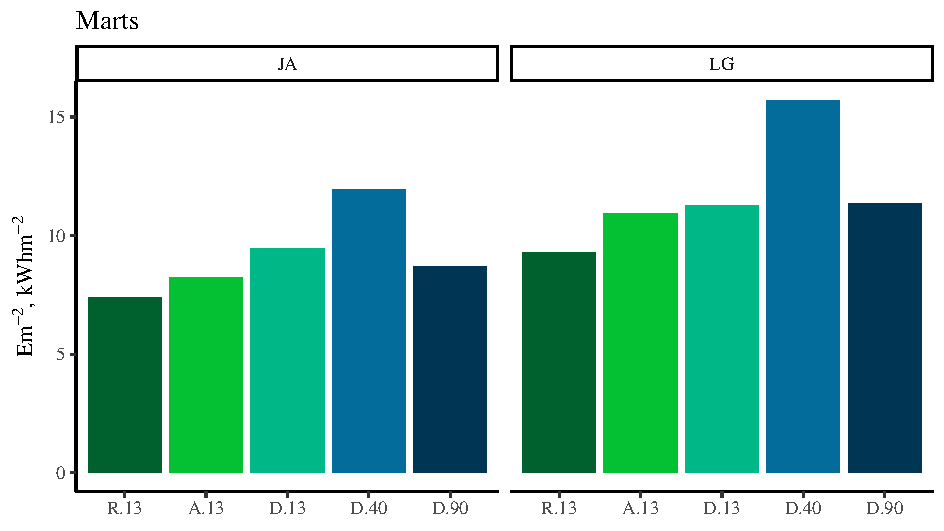
\includegraphics[width=\linewidth]{figures/sol_month/mar_m_m2.pdf}
%     \caption{Saules paneļu saražotā enerģija martā}
%     \label{fig:mar_sum}
% \end{figure}

\begin{figure}[h]
    \centering
    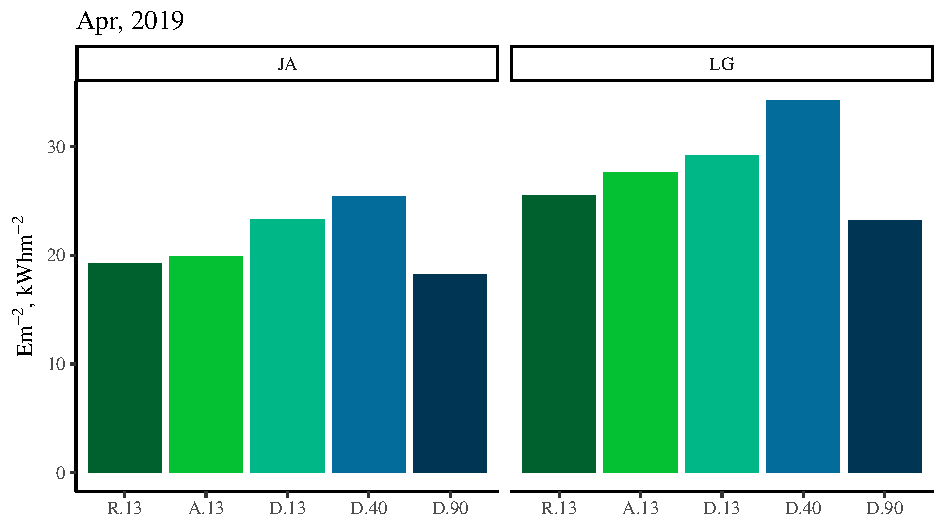
\includegraphics[width=\linewidth]{figures/sol_month/apr_m_m2.pdf}
    \caption{Saules paneļu saražotā enerģija aprīlī}
    \label{fig:apr_sum}
\end{figure}


% \subsection{Efektivitāte}\label{subsection:effectivity}

% Izmērītā paneļu efektivitāte atšķiras no ražotāju tehniskajā dokumentācijā dotā. Atšķirības tiek skaidrotas ar efektivitātes mērīšanas veidu -- standarta testi tiek veikti pie konstanta izstarojuma (1000 W/m$^2$ un 800 W/m$^2$), tomēr reālā poligona apstākļos saņemtais starojums ir mainīgs.
% % Iespējams tāpēc, ka visu paneļu saules apstarojuma references punktu izvēlējos eksperimentālā poligona meteostacijas datus un nepiereizināju tiem panelim atbilstošo leņķi, jo saules apstarojums mainās no leņķa.
% % you better do it fast 
% \begin{figure}[h]
%     \centering
%     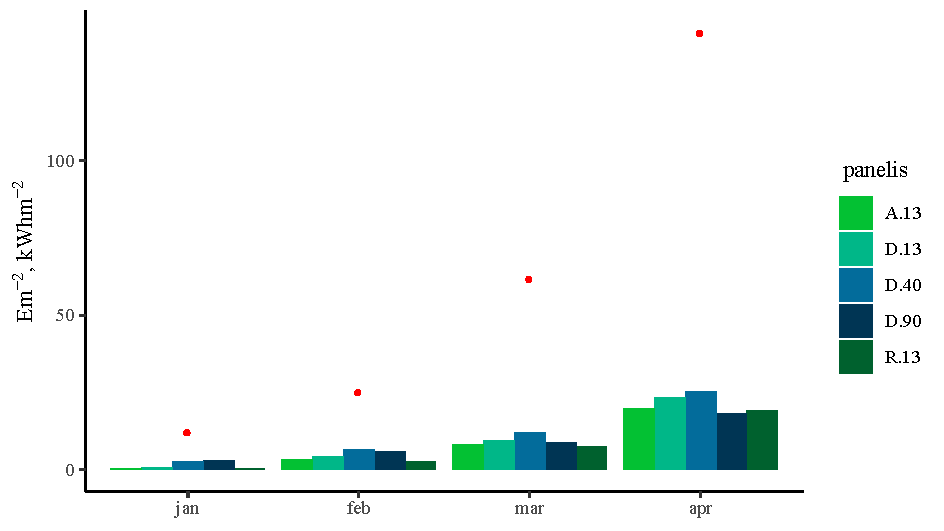
\includegraphics[width=\linewidth]{figures/results/ja_m2.pdf}
%     \caption{JA tipa paneļu saražotais mēnesī salīdzinājumā ar eksperimentālā poligona meteostacijas stacijas saules apstarojuma datiem (sarkanā krāsā)}
%     \label{fig:ja}
% \end{figure}
% \begin{table}[h]
%     \caption{JA tipa paneļu efektivitāte procentos}
%     \begin{center}
%     %%%%%%%%%%%%%%%%%%%%%%%%%%%%%%%%%%%%%%%%%%%%%%%%%%%%%%%%%%%%%%%%%%%%%%
%%                                                                  %%
%%  This is a LaTeX2e table fragment exported from Gnumeric.        %%
%%                                                                  %%
%%%%%%%%%%%%%%%%%%%%%%%%%%%%%%%%%%%%%%%%%%%%%%%%%%%%%%%%%%%%%%%%%%%%%%
\begin{tabular}{ | c | c c c c c | } \hline
E, $\%$	&A.13	&R.13	&D.13	&D.40	&D.90\\ \hline
jan	&2.86	&1.87		&5.90	&20.27	&23.08\\
feb	&12.72	&10.91		&16.97	&25.65	&23.82\\
mar	&13.31	&11.98		&15.34	&19.33	&14.11\\
apr	&14.06	&13.60		&16.45	&17.98	&12.91\\ \hline
vid	&10.74	&9.59		&13.67	&20.81	&18.48\\ \hline
\end{tabular}
%     \end{center}
%     \label{tab:JA_eff}
% \end{table}

% \begin{figure}[h]
%     \centering
%     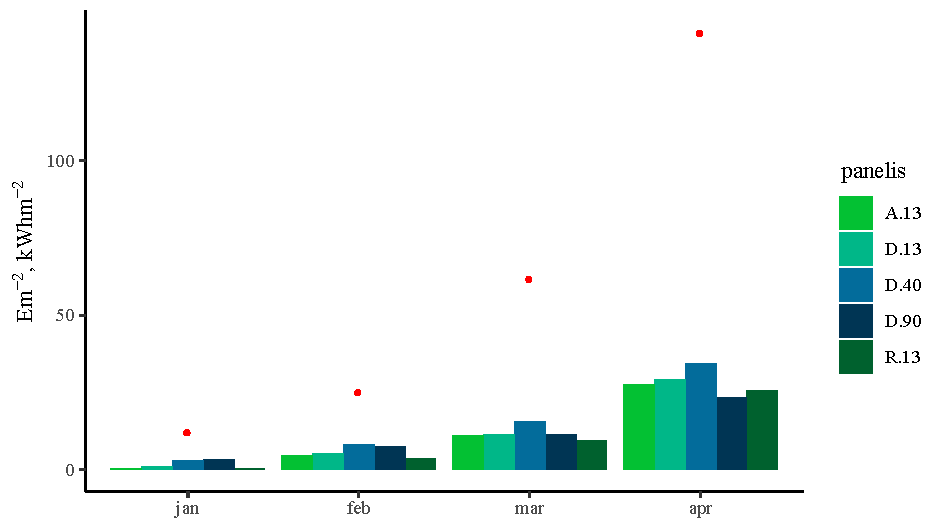
\includegraphics[width=\linewidth]{figures/results/lg_m2.pdf}
%     \caption{LG tipa paneļu saražotais mēnesī salīdzinājumā ar eksperimentālā poligona meteostacijas stacijas saules apstarojuma datiem (sarkanā krāsā)}
%     \label{fig:lg}
% \end{figure}
% \begin{table}[h]
%     \caption{LG tipa paneļu efektivitāte procentos}
%     \begin{center}
%     %%%%%%%%%%%%%%%%%%%%%%%%%%%%%%%%%%%%%%%%%%%%%%%%%%%%%%%%%%%%%%%%%%%%%%
%%                                                                  %%
%%  This is a LaTeX2e table fragment exported from Gnumeric.        %%
%%                                                                  %%
%%%%%%%%%%%%%%%%%%%%%%%%%%%%%%%%%%%%%%%%%%%%%%%%%%%%%%%%%%%%%%%%%%%%%%
\begin{tabular}{ | c | c c c c c | }\hline
E, $\%$	&A.13	&R.13	&D.13	&D.40	&D.90\\ \hline
jan		&4.1	&2.9	&7.8	&23.2	&26.5\\
feb		&17.6	&14.4	&20.1	&32.8	&29.5\\
mar		&17.7	&15.0	&18.2	&25.4	&18.4\\
apr		&19.5	&18.0	&20.6	&24.2	&16.4\\ \hline
vid		&14.7	&12.6	&16.7	&26.4	&22.7\\ \hline
\end{tabular}
%     \end{center}
%     \label{tab:LG_eff}
% \end{table}


%* Secinājumi
\chapter*{Secinājumi}
\addcontentsline{toc}{chapter}{Secinājumi}
Darba laikā tika izveidota programmatūra, ar kuras palīdzību tika atlasīts, analizēts un apkopots liels datu apjoms par 10 saules paneļu darbību no 2019. gada 1. janvāra līdz 30. aprīlim. Pētījuma datu analīzes rīks ir pieejams \url{https://github.com/chararchter/solR}.

Darbā iegūtie rezultāti ļauj izdarīt secinājumus, ka no sistēmā esošajiem parametriem efektīvākā kombinācija ir:
\begin{itemize}
	\item 40 grādu leņķis
	\item D virziens
	\item LG panelis
	\item aprīļa mēnesis
\end{itemize}

% KĻŪDAS!!!?????????

Saules paneļu efektivitātes citu faktoru ietekmes izpratne prasa turpmākus pētījumus, it īpaši nolietojuma, putekļu, vēja, nokrišņu un citu apstākļu ietekmes izvērtēšanai. Lai iegūtu datus un veiktu analīzi pilna gada periodam, šo montiroingu ir paredzēts turpināt vismaz trīs gadus.

%* Pateicības
\chapter*{Pateicības}
\addcontentsline{toc}{chapter}{Pateicības}
Pateicos paroksetīnam, xanax, GNU/Linux, Pētera Draguna dzejas krājumam 'Tumšās stundas', Tarvi Verro for teaching me git, Valtam Krūmiņam un Annai Bulei par emocionālo atbalstu, Paulīnai Lodbrukai un Pēterim Ratniekam par ticību maniem spēkiem, Žeņam par kucēnu video, Solvitai par maģiju un Cilvēkam par pacietību. Paldies Aleksandrai Elbakjanai par sci-hub. Paldies "Puratos Latvia" un Asjas un Berndta Everts piemiņas fondam par stipendiju studiju laikā.\\

Darbs veikts ar Eiropas Reģionālās attīstības fonta projekta "Viedo risinājumu gandrīz nulles enerģijas ēkām izstrāde, optimizācija un ilgtspējas izpēte reāla klimata apstākļos" Nr ESS2017/209 1.1.1.1/16/A/192 finansiālo atbalstu.


%* Izmantotā darba literatūra un avoti
\clearpage
\addcontentsline{toc}{chapter}{Izmantotā darba literatūra un avoti}
\printbibliography[title=Izmantotā darba literatūra un avoti]

%%% Pielikumi
\appendix

% Dokumentālā lapa
\makedoklapa

\end{document}
